\documentclass[a4paper,10pt]{article}
\usepackage[T1]{fontenc}
\usepackage[utf8]{inputenc}
\usepackage{palatino}
\usepackage{fullpage}
\usepackage{graphicx}
\usepackage{float}
\renewcommand{\arraystretch}{1.1}

\title{{\large{COMPSCI 597: Big Data and NOSQL Databases}}\\Term Project Final Report}
\author{Tanner, Reuben, Trisca, Gabriel}
\begin{document}

\maketitle

\tableofcontents

\newpage

\section{Introduction}
\subsection{Motivation}
Cities and communities maintain databases of crime to be able to predict and prevent criminal activities from happening. A major motivation behind what is called “crime data mining” \cite{Blockeel2013} is identifying patterns of criminal behavior\cite{Chen2004}. 

Crime is a big burden on society: in the United States alone, 23 million criminal offenses were committed in 2007. The economic loss of victims was \$15 billion and \$179 billion were spent by the government on police protection, judicial and legal activities, and corrections \cite{Justice2008}. Even if a small percentage of these crimes can be prevented, the impact would be extremely significant\cite{Syam2006}.

In addition, identifying what variables influence the likelihood of a certain type of crime happening can shed light on the complex dynamics behind all criminal behavior, helping understand the motivations behind these antisocial conducts, and how the environment affects people and the choices they make\cite{BUSS2012}.

\subsection{Dataset}
We are working with four datasets:
\begin{description}
	\item[Weather] Daily weather summaries from the City of Chicago for the time period 2001 – 2013 \\\textit{Location: http://www.ncdc.noaa.gov/cdo-web/}
	
	\item[Crime] This dataset reflects reported incidents of crime (with the exception of murders where data exists for each victim) that occurred in the City of Chicago from 2001 to present, minus the most recent seven days. Data is extracted from the Chicago Police Department's CLEAR (Citizen Law Enforcement Analysis and Reporting) system. \\\textit{Location: https://data.cityofchicago.org/Public-Safety/Crimes-2001-to-present/ijzp-q8t2}
	
	\item[Socioeconomic Indicators] Census Data - Selected socioeconomic indicators in Chicago, 2007 – 2011 \\\textit{Location: https://data.cityofchicago.org/Health-Human-Services/Census-Data-Selected-socioeconomic-indicators-in-C/kn9c-c2s2}
	
	\item[Public Health Statistics] Selected public health indicators by Chicago community area.\\\textit{Location: https://data.cityofchicago.org/Health-Human-Services/Public-Health-Statistics-Selected-public-health-in/iqnk-2tcu}
	
\end{description}


\section{Problem}
We want to predict crime by using socio-economical information, health indicators for the different areas in which crimes are committed and historical weather information collected in the city of Chicago. 

\section{Method}

\subsection{Code Structure}

With our focus in mind of being able to predict crimes, we needed a glue that would allow us to connect our socio-economic indicators, public health indicators, weather and crime data. The "community area" ended up being the exact glue that we needed. Chicago is broken up into 77 community areas and, in each of our datasets (aside from weather) the community area is either explicitly or implicitly defined. 

The first phase of our analysis was to map each crime to a community area based on its specified latitude and longitude. This involved finding a KML file which contained the boundaries for each of the 77 community areas and then generating polygons for each of the community areas and mapping each crime to its corresponding polygon. Once we had successfully mapped each crime to a community area, we remapped the entire dataset to a file, stripping the unnecessary fields of the crimes and applying the community areas.\\

Once we had remapped the dataset to only contain the fields we needed and the one we extrapolated we were ready to begin focusing on the relationships. Because of the abundance of different crime types (384 specifically), we decided that attempting to derive correlations for each of them would be somewhat fruitless so we narrowed our focus to be only on the top 50 crimes committed over the entire city. This data was extracted by one simple Hadoop job. 


After determining which crimes occurred frequently and which community areas they occurred in we had enough information to extract correlations from public health indicators and socio-economic indicators but we still needed a way to link crimes to our weather dataset which listed the weather daily. We decided this could best be accomplished by running a job to determine what crimes (of the top 50) occurred on any given day so the dataset was remapped to have a key of a day and a value of the frequencies of the top 50 crimes committed on that day.\\
	

At this point, we had enough pieces of data to link all of our datasets and now we needed to determine which of them were correlated with which others so we pulled out the big guns and wrote a manual full join against each of the files and the crime dataset. This was especially challenging considering there were 4 files being joined and one of the files (the weather dataset) required a different matching scheme than the public health indicators and the socio-economic indicators because weather was keyed by date. In the reduce phase of the correlation, x, y points were calculated for crime type and frequency vs. severity of public health indicator, crime type and frequency vs. severity of economic indicator and crime type and frequency vs. weather pattern. A file was produced containing the points for each of the features within the each of the files.

\subsection{Challenges}
One of our initial challenges that we faced was our choice of data set. When we first began this project we desired to perform analytics on a crime dataset for Washington DC to perform geospatial and temporal analysis. Once we started getting into the dataset that was on the opendata website for DC, we realized that the data did not have accurate locations provided through latitude and longitude or through any other means so we decided to go with a different dataset that we could more easily plot, specifically, the 311 requests dataset from Washington DC.

After we shifted our focus from crime to the 311 requests, we began performing analysis on it by following the pattern laid out in our Data Analysis section. After we generated scatter plots and correlations for the requests against weather patterns and begin critically examining them, much to our dismay, we found that there were very few interesting correlations. One of the most obvious and mundane correlations we found was that on cold days there are more requests for heating; ground breaking.\\

Once we reached the dead end with the 311 requests we decided to switch our focus to finding a new, crime dataset that would have the features which would make the analysis far more interesting. Our paper is written about that dataset, namely, the Chicago crimes dataset.

\subsection{Data Analysis}
In order to calculate correlation between different datasets, we needed a common column or key between them.

\begin{table}
	\begin{tabular}{|c|l|}
	\hline 
	\textbf{Indicator Name} & \textbf{Description} \\ 
	\hline 
	16\_UNEMPLOYED & Percentage of persons 16 or older and unemployed \\\hline
25\_NO\_HIGHSCHOOL & Percentage of persons 25 or older without a high school diploma \\\hline
BELOW\_POVERTY & Percentage of persons under the federal poverty line\\\hline
BLOOD\_LEAD & Micrograms of lead in blood\\\hline
CANCER & Cancer rates per 10,000 people\\\hline
CROWDED & Percentage of people living in crowded housing environments\\\hline
INCOME & Average income level\\\hline
LOW\_BIRTH\_WEIGHT & Percentage of babies being born with weight under normal level\\\hline
NO\_HIGHSCHOOL & Percentage of persons without a high school diploma\\\hline
PRENATAL\_CARE & Percentage of children that received prenatal care\\\hline
PRETERM\_BIRTH & Percentage of children born prematurely\\\hline
TEEN\_BIRTH & Rate of teen pregnancy and birth\\\hline
UNEMPLOYMENT & Unemployment rate (percentage)\\\hline
YOUNG\_OR\_OLDER & Percentage of poersons 16 or younger and 65 or older \\
\hline
	\end{tabular} 
	\caption{Indicators and their description}
\end{table}

As an initial step, we are calculating the correlation between crime frequency and different indicators. To achieve this, we performed a join operation between the weather data and the crime frequency data with date as the key. For the socio-economic and public health indicators we joined the datasets on the community area where the statistics came from and where the crime was committed, and the crime frequency was accumulated.\\

These scatter plots are the top most highly correlated pairs of indicator/crime type.\\
\begin{figure}[H]
\centering
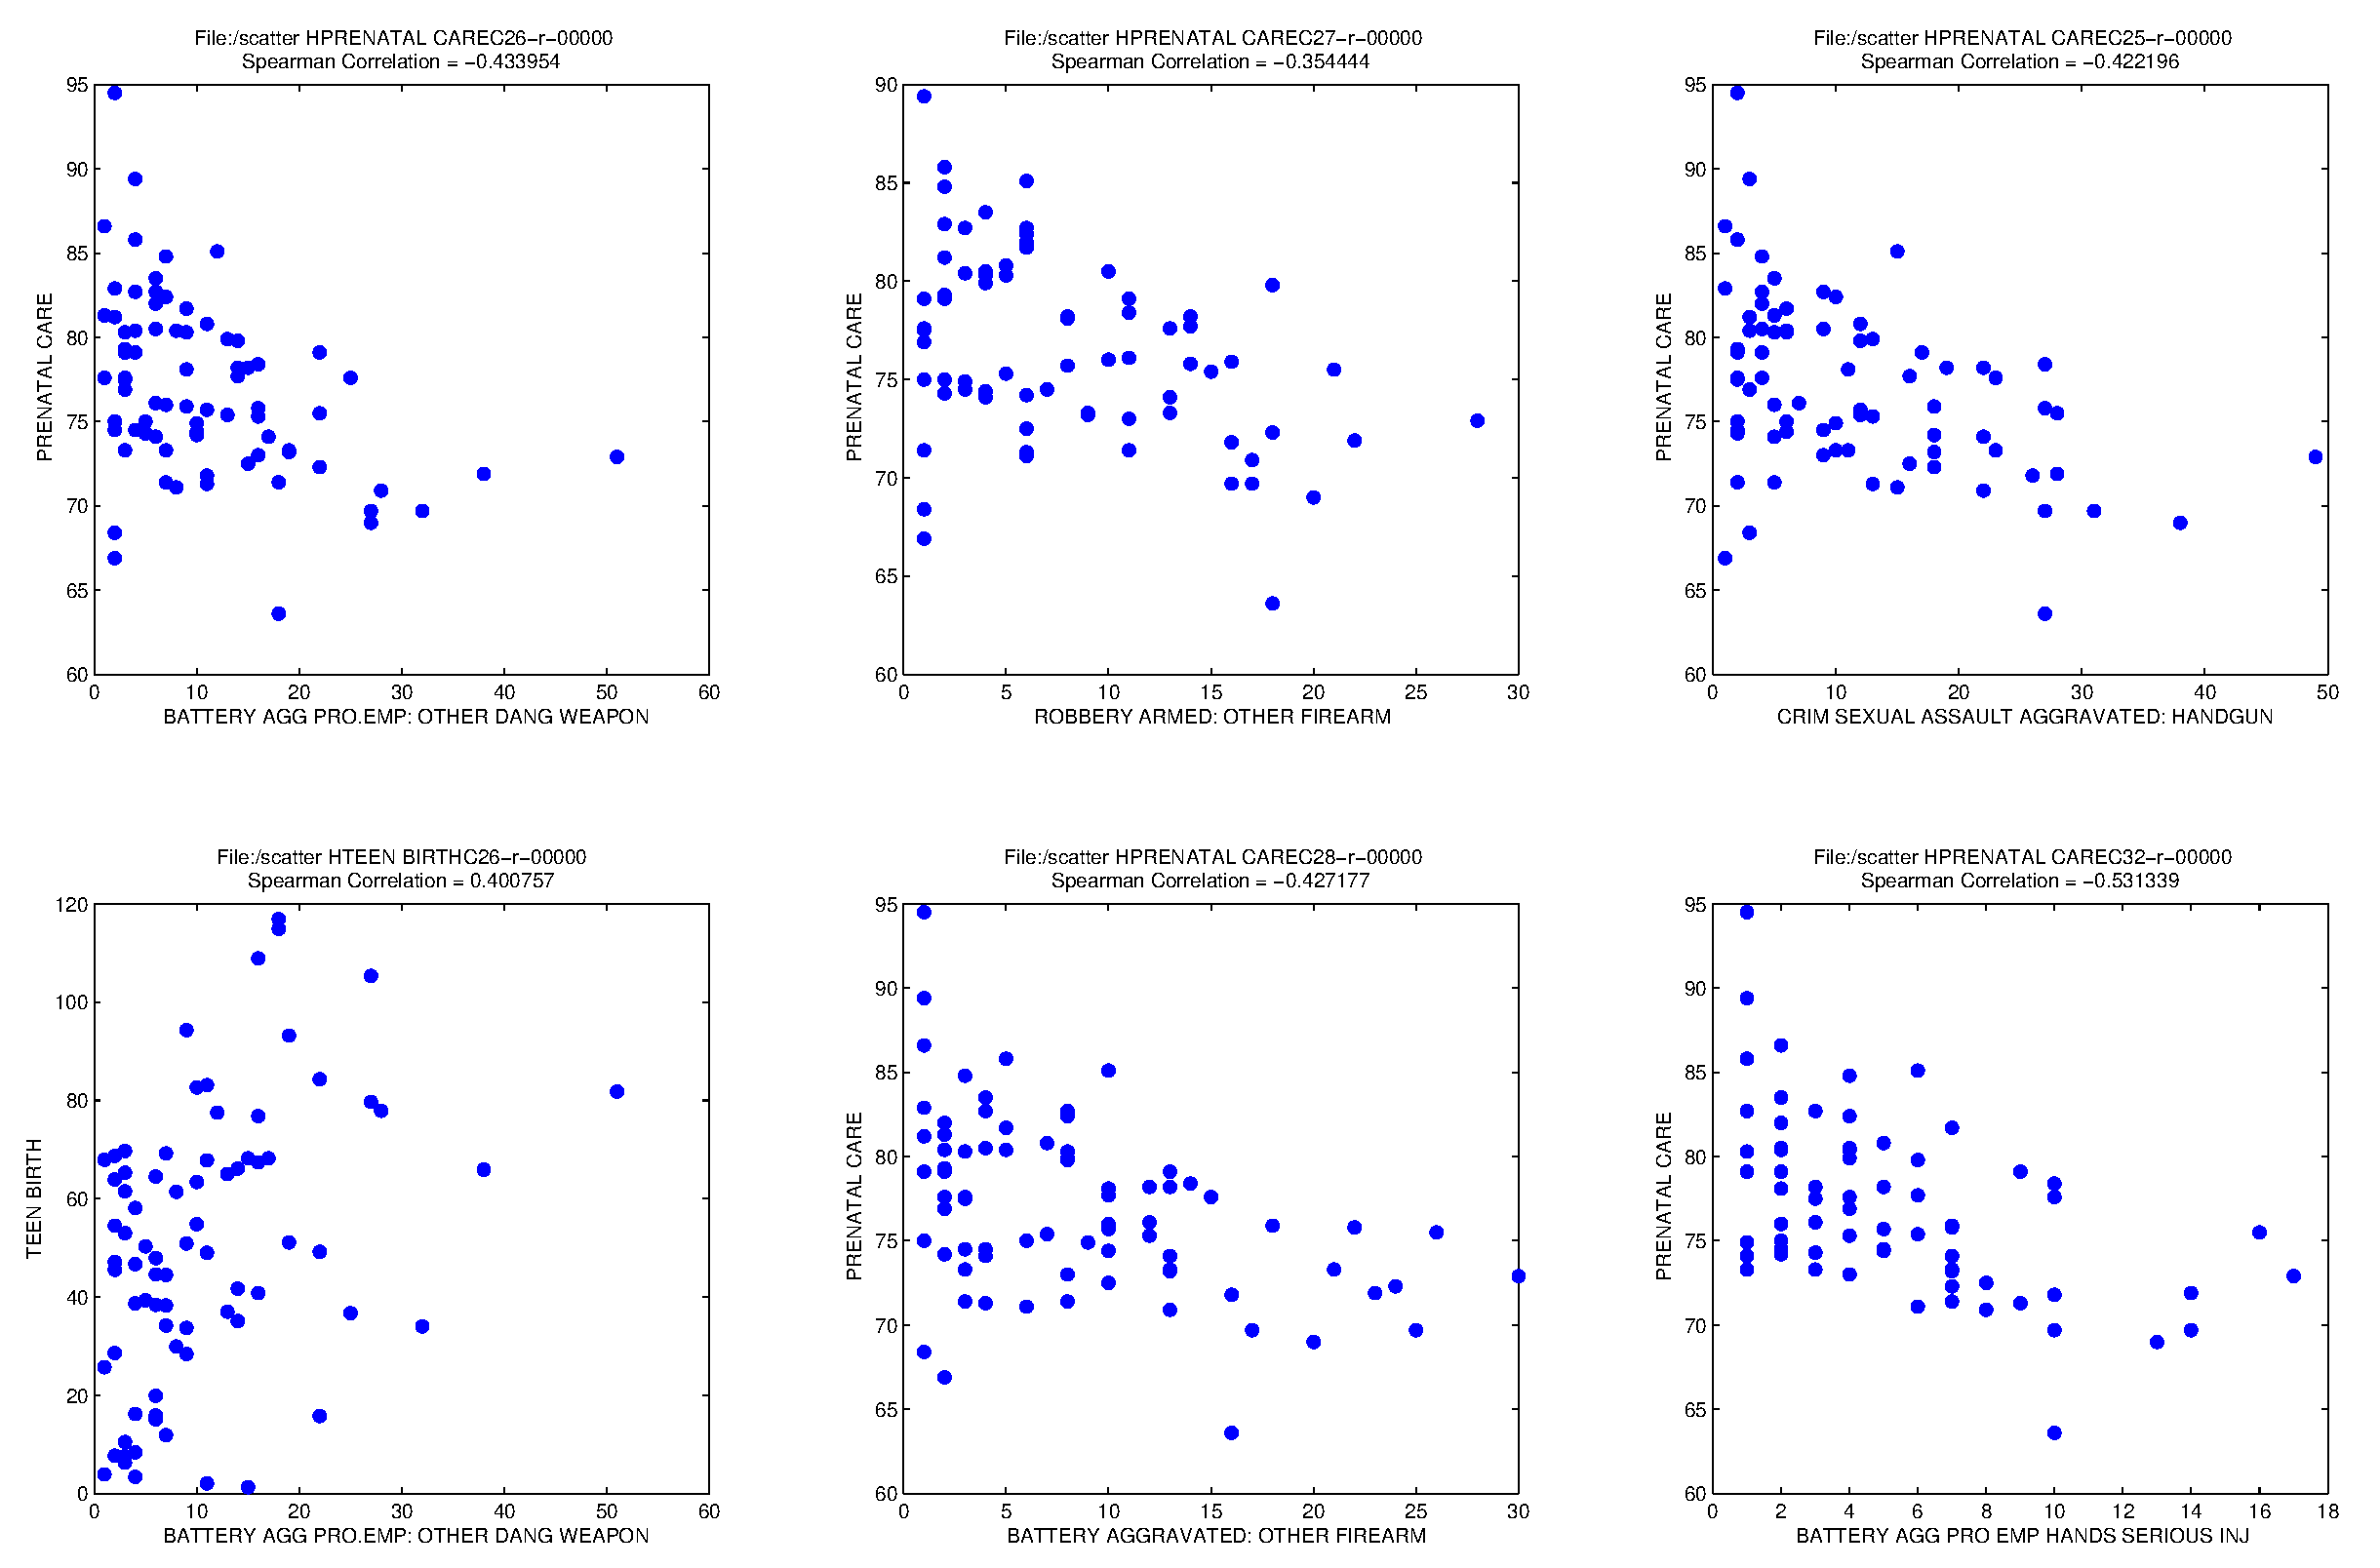
\includegraphics[width=0.8\linewidth]{media/ScatterPlot1.eps}\hfill
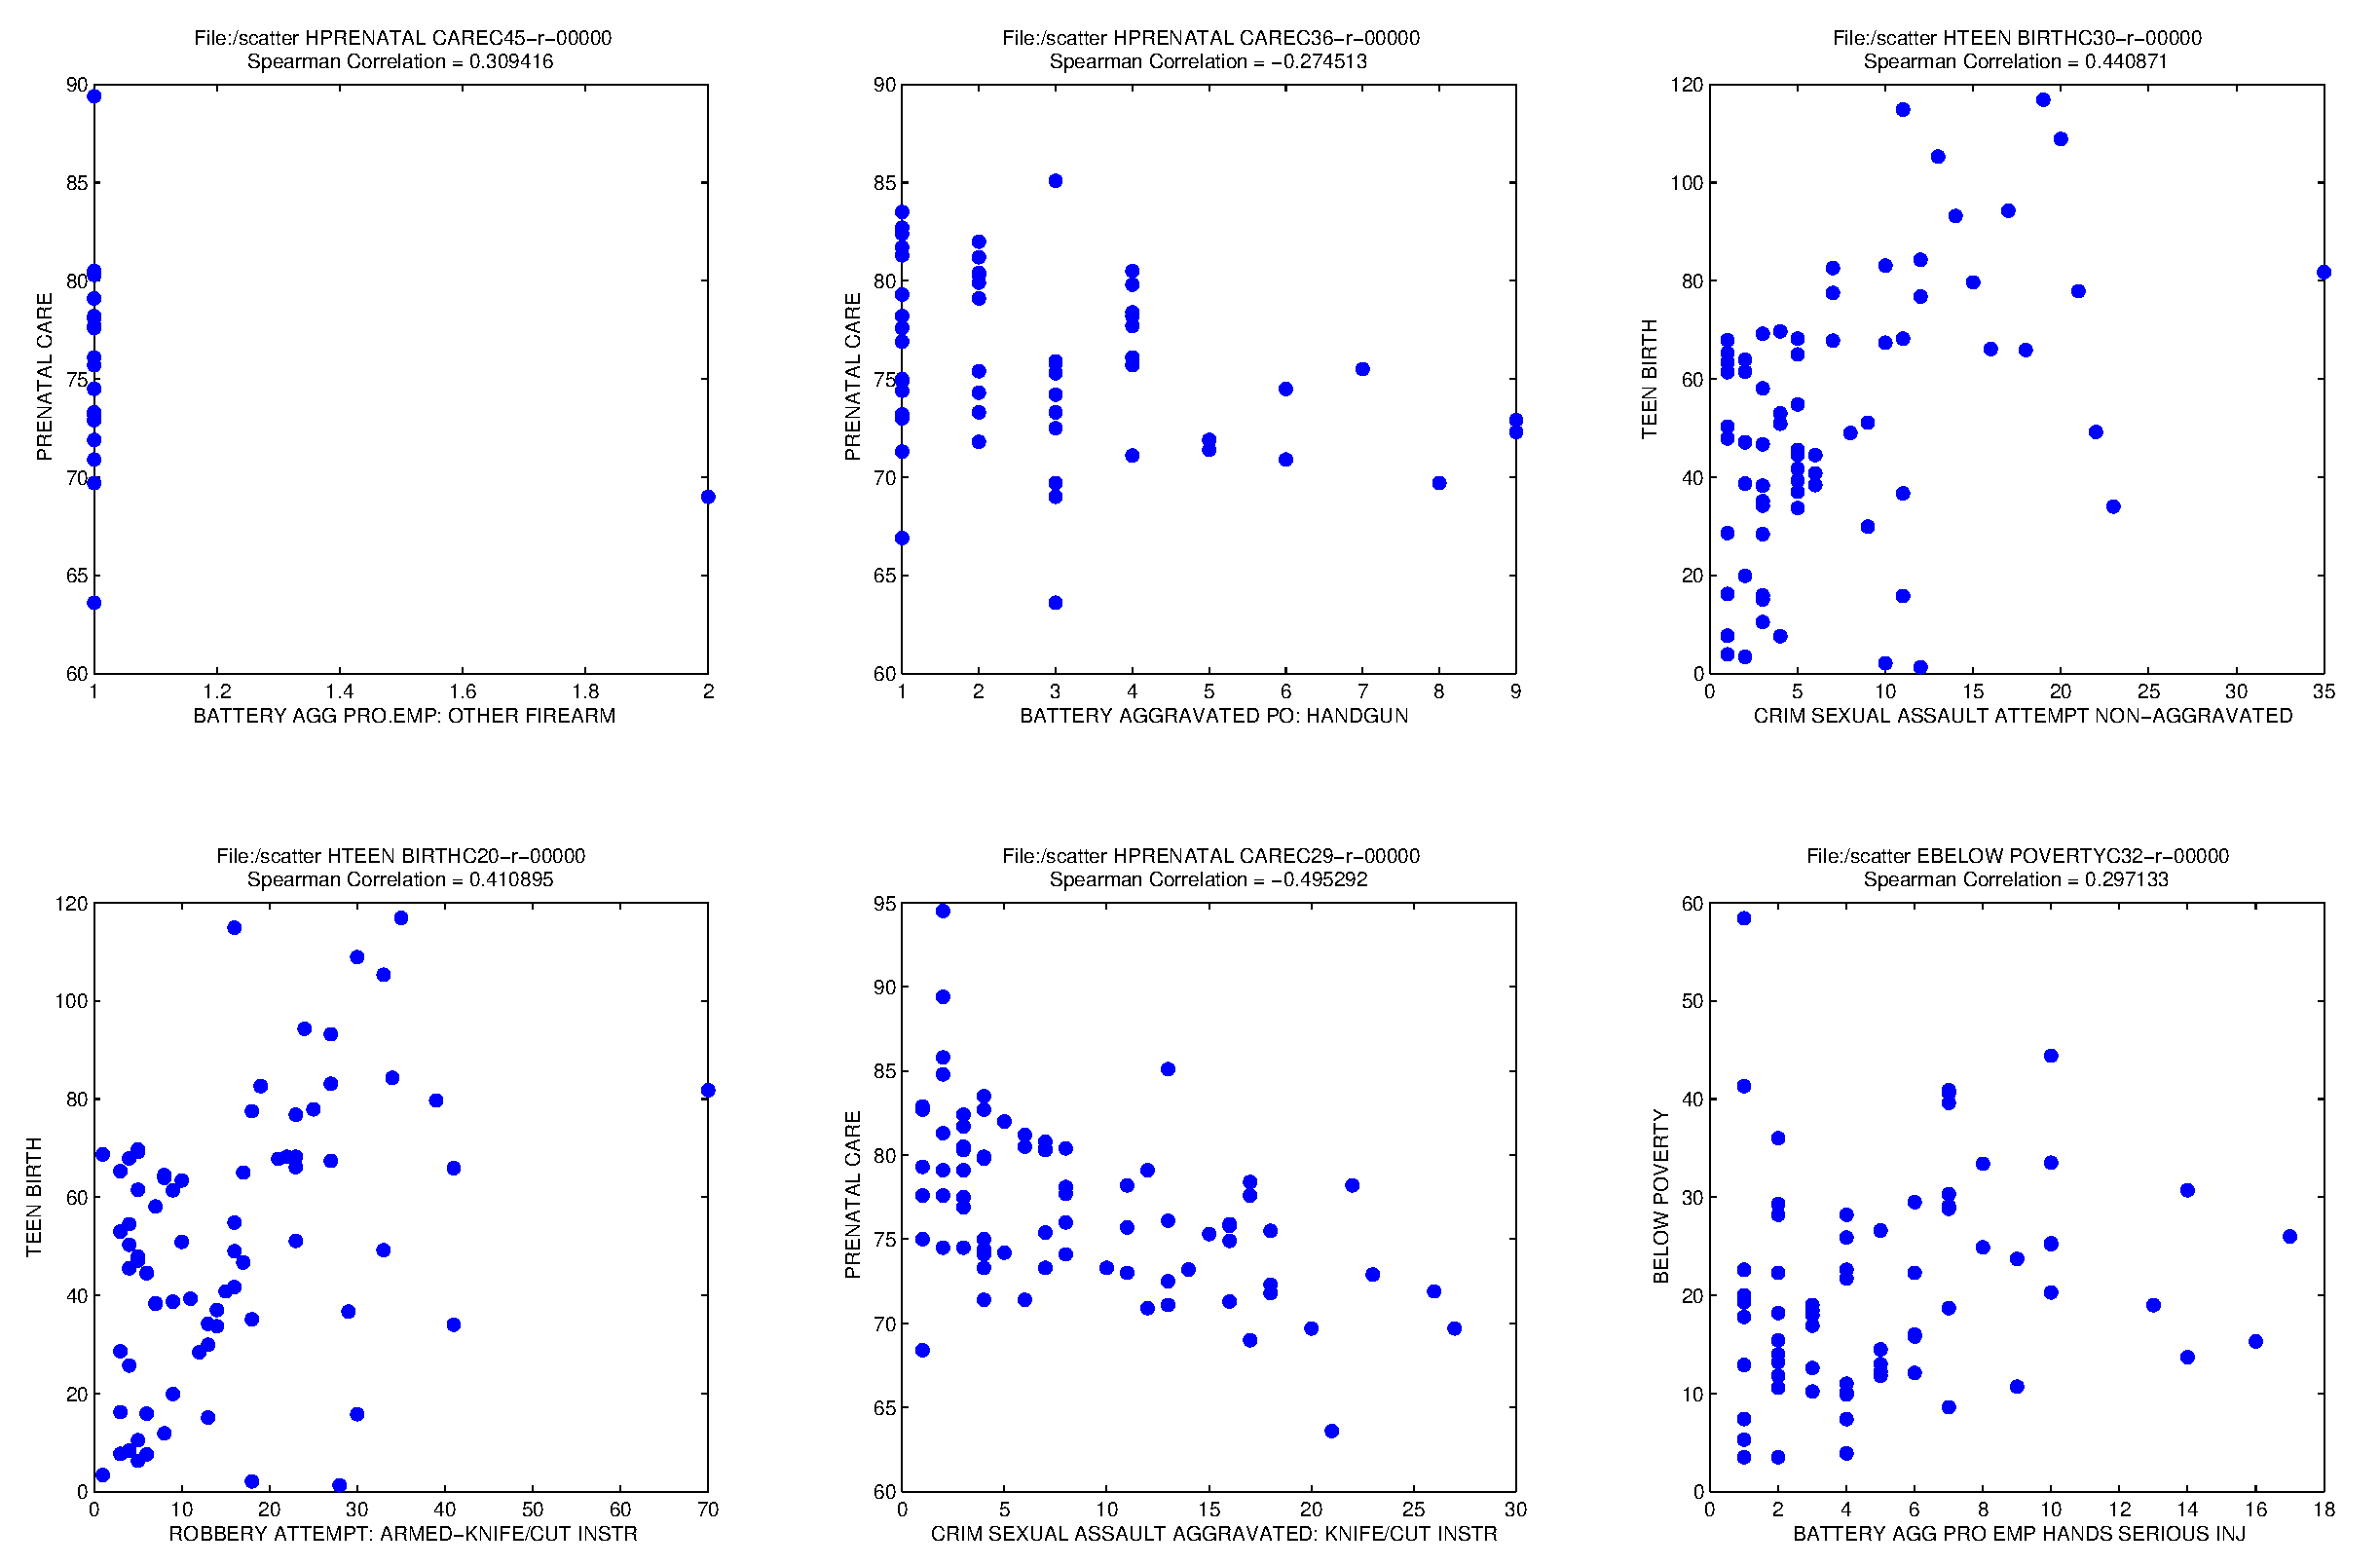
\includegraphics[width=0.3\linewidth]{media/ScatterPlot2.eps}
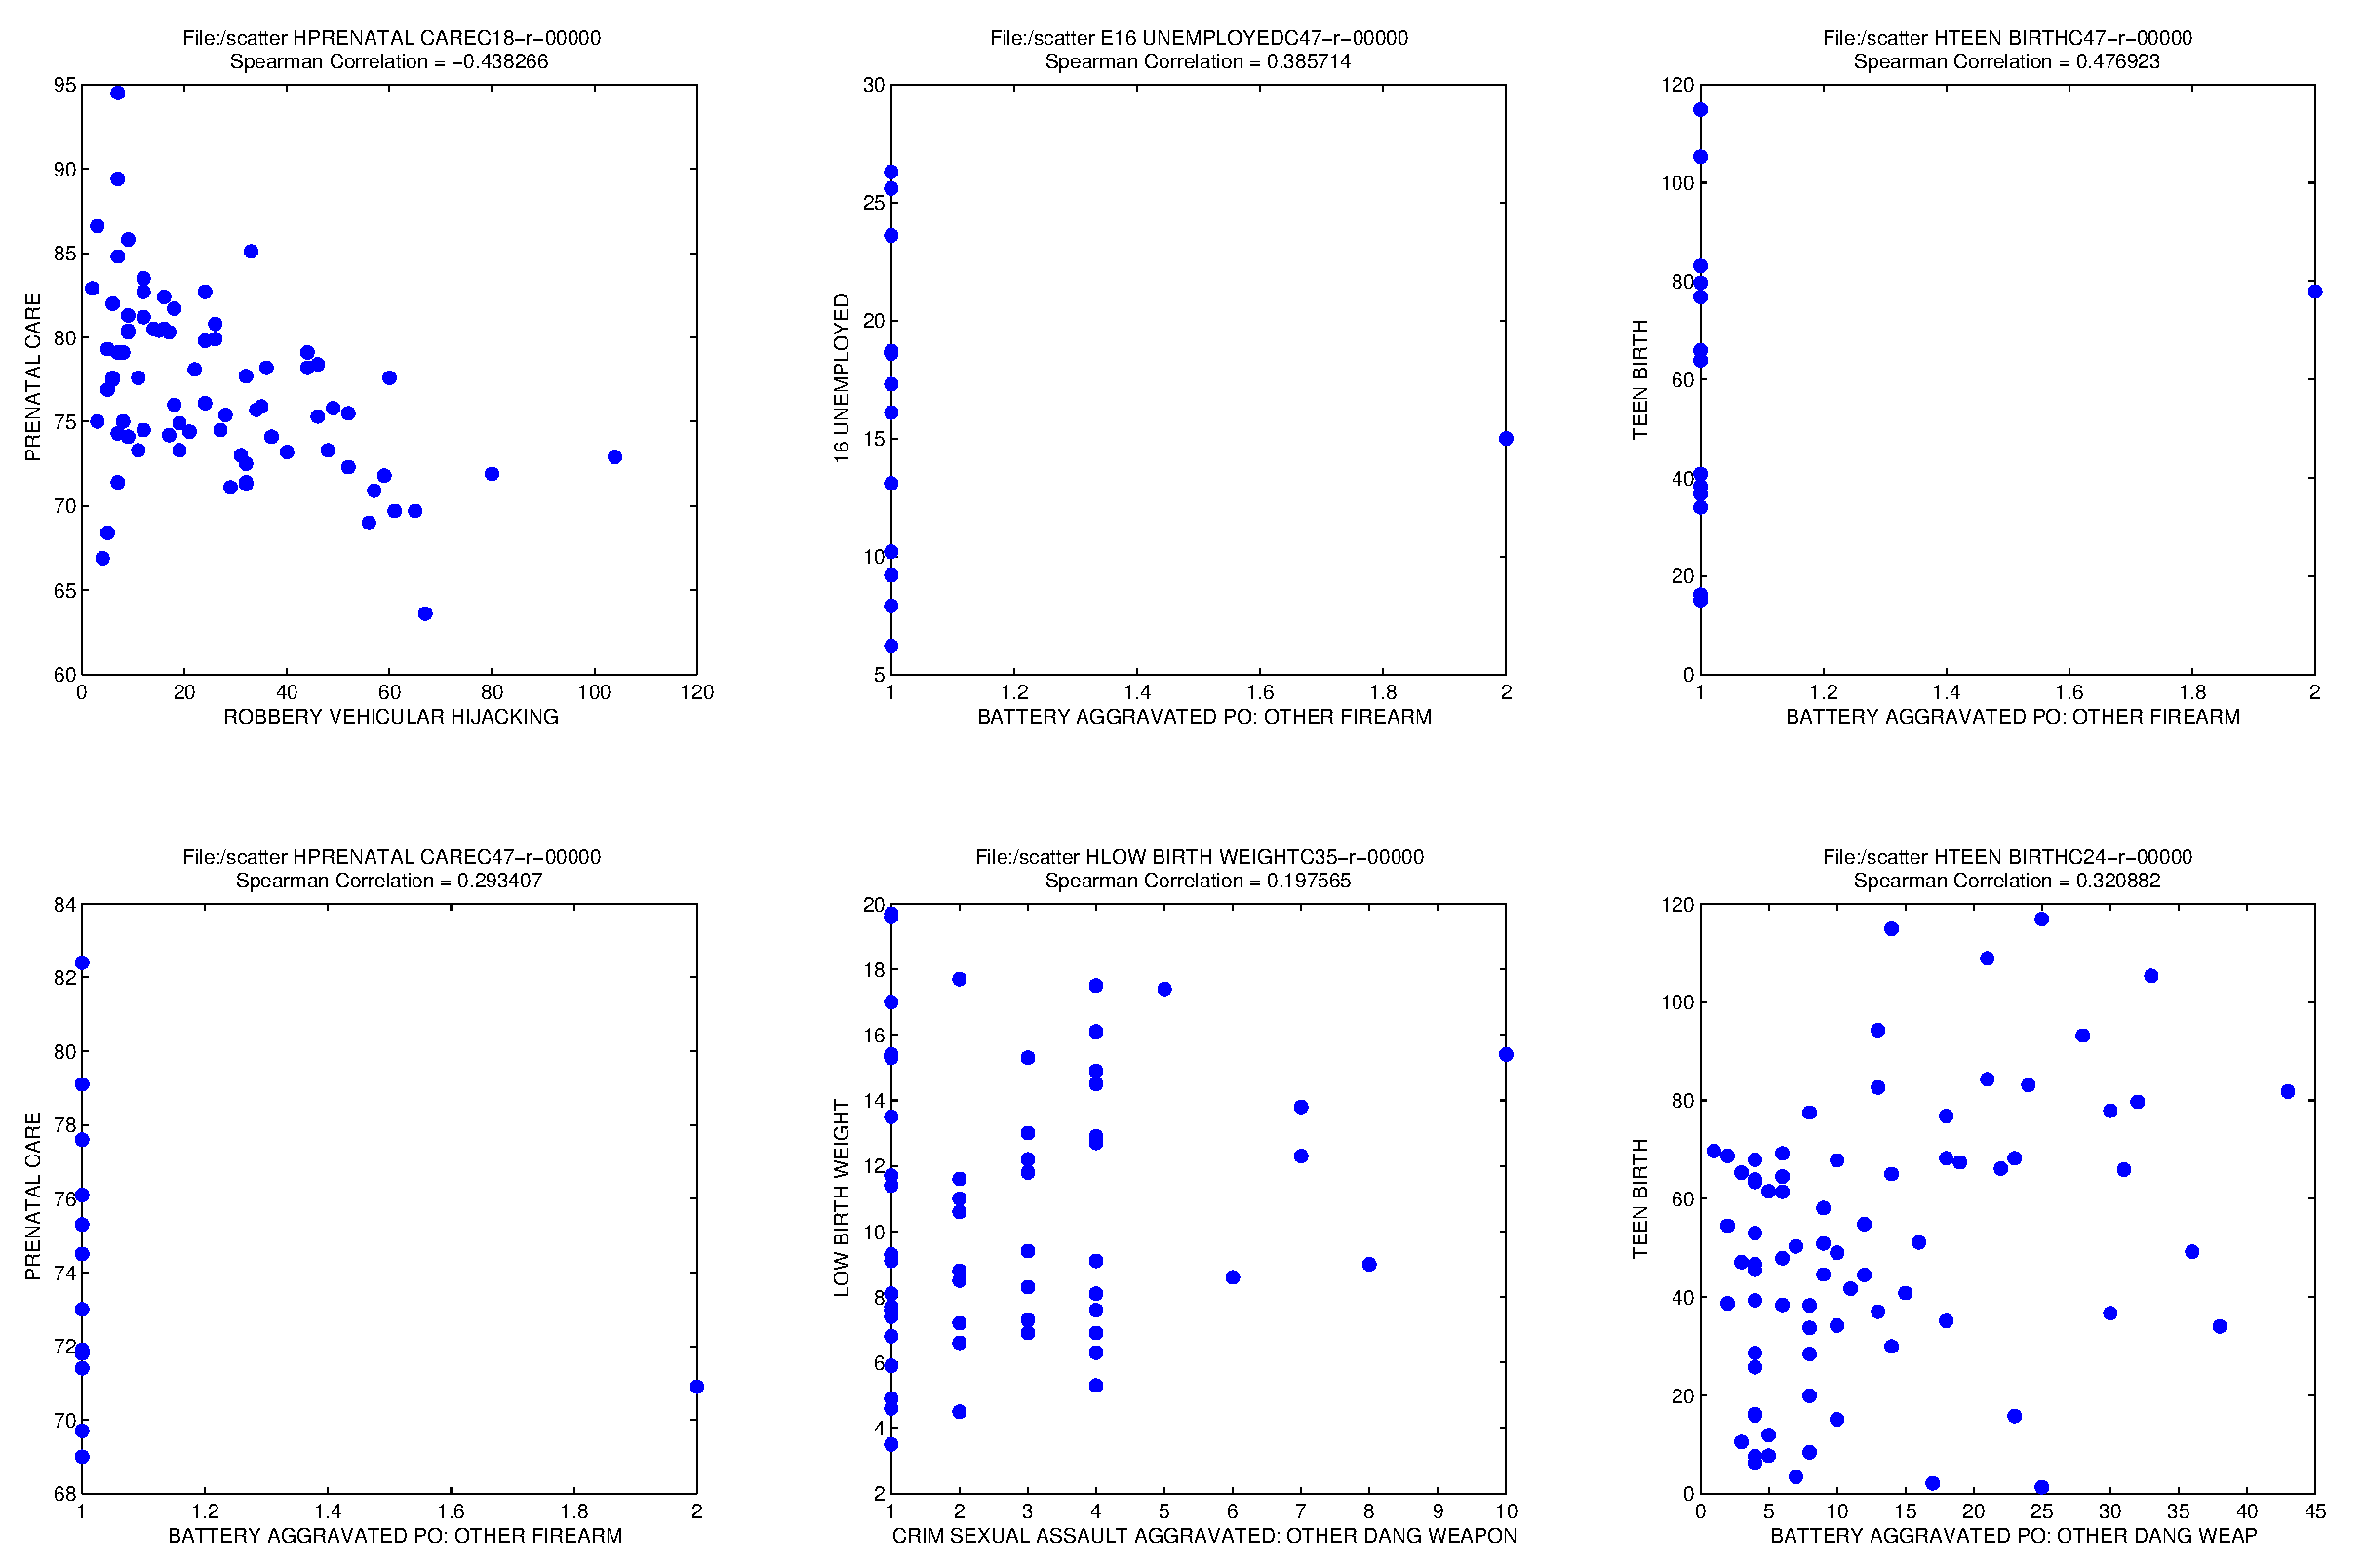
\includegraphics[width=0.3\linewidth]{media/ScatterPlot3.eps}
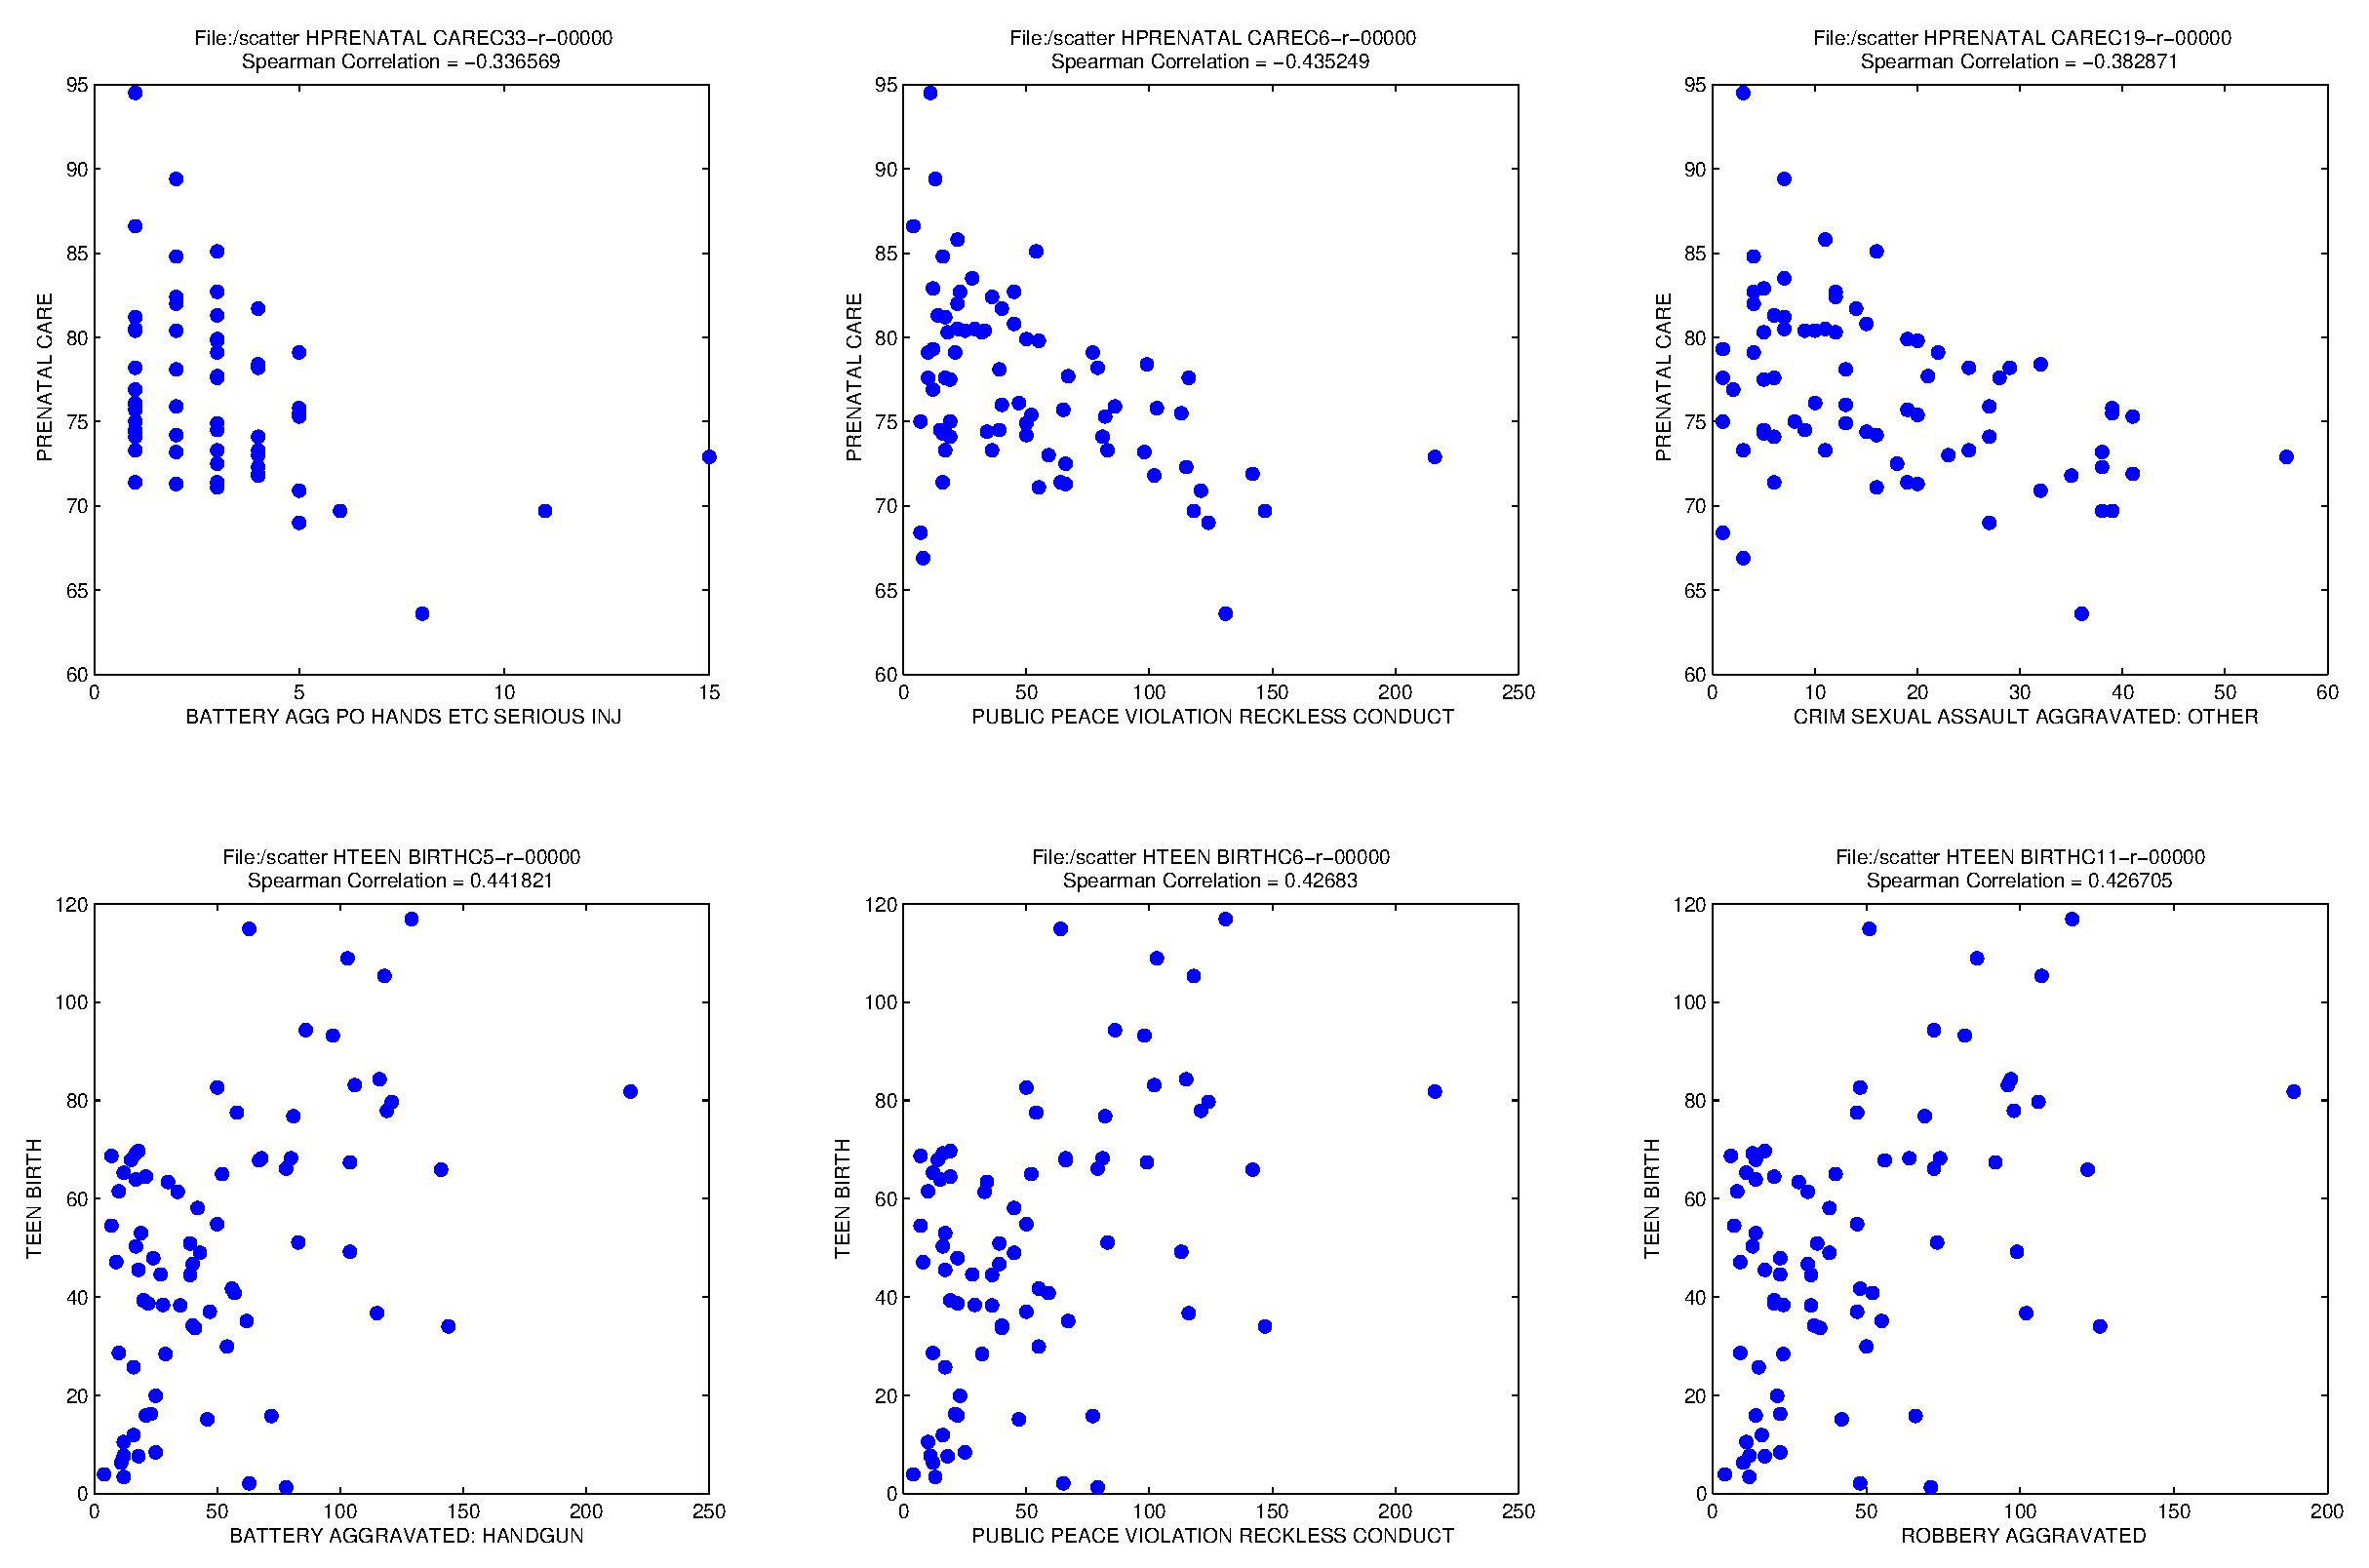
\includegraphics[width=0.3\linewidth]{media/ScatterPlot4.eps}
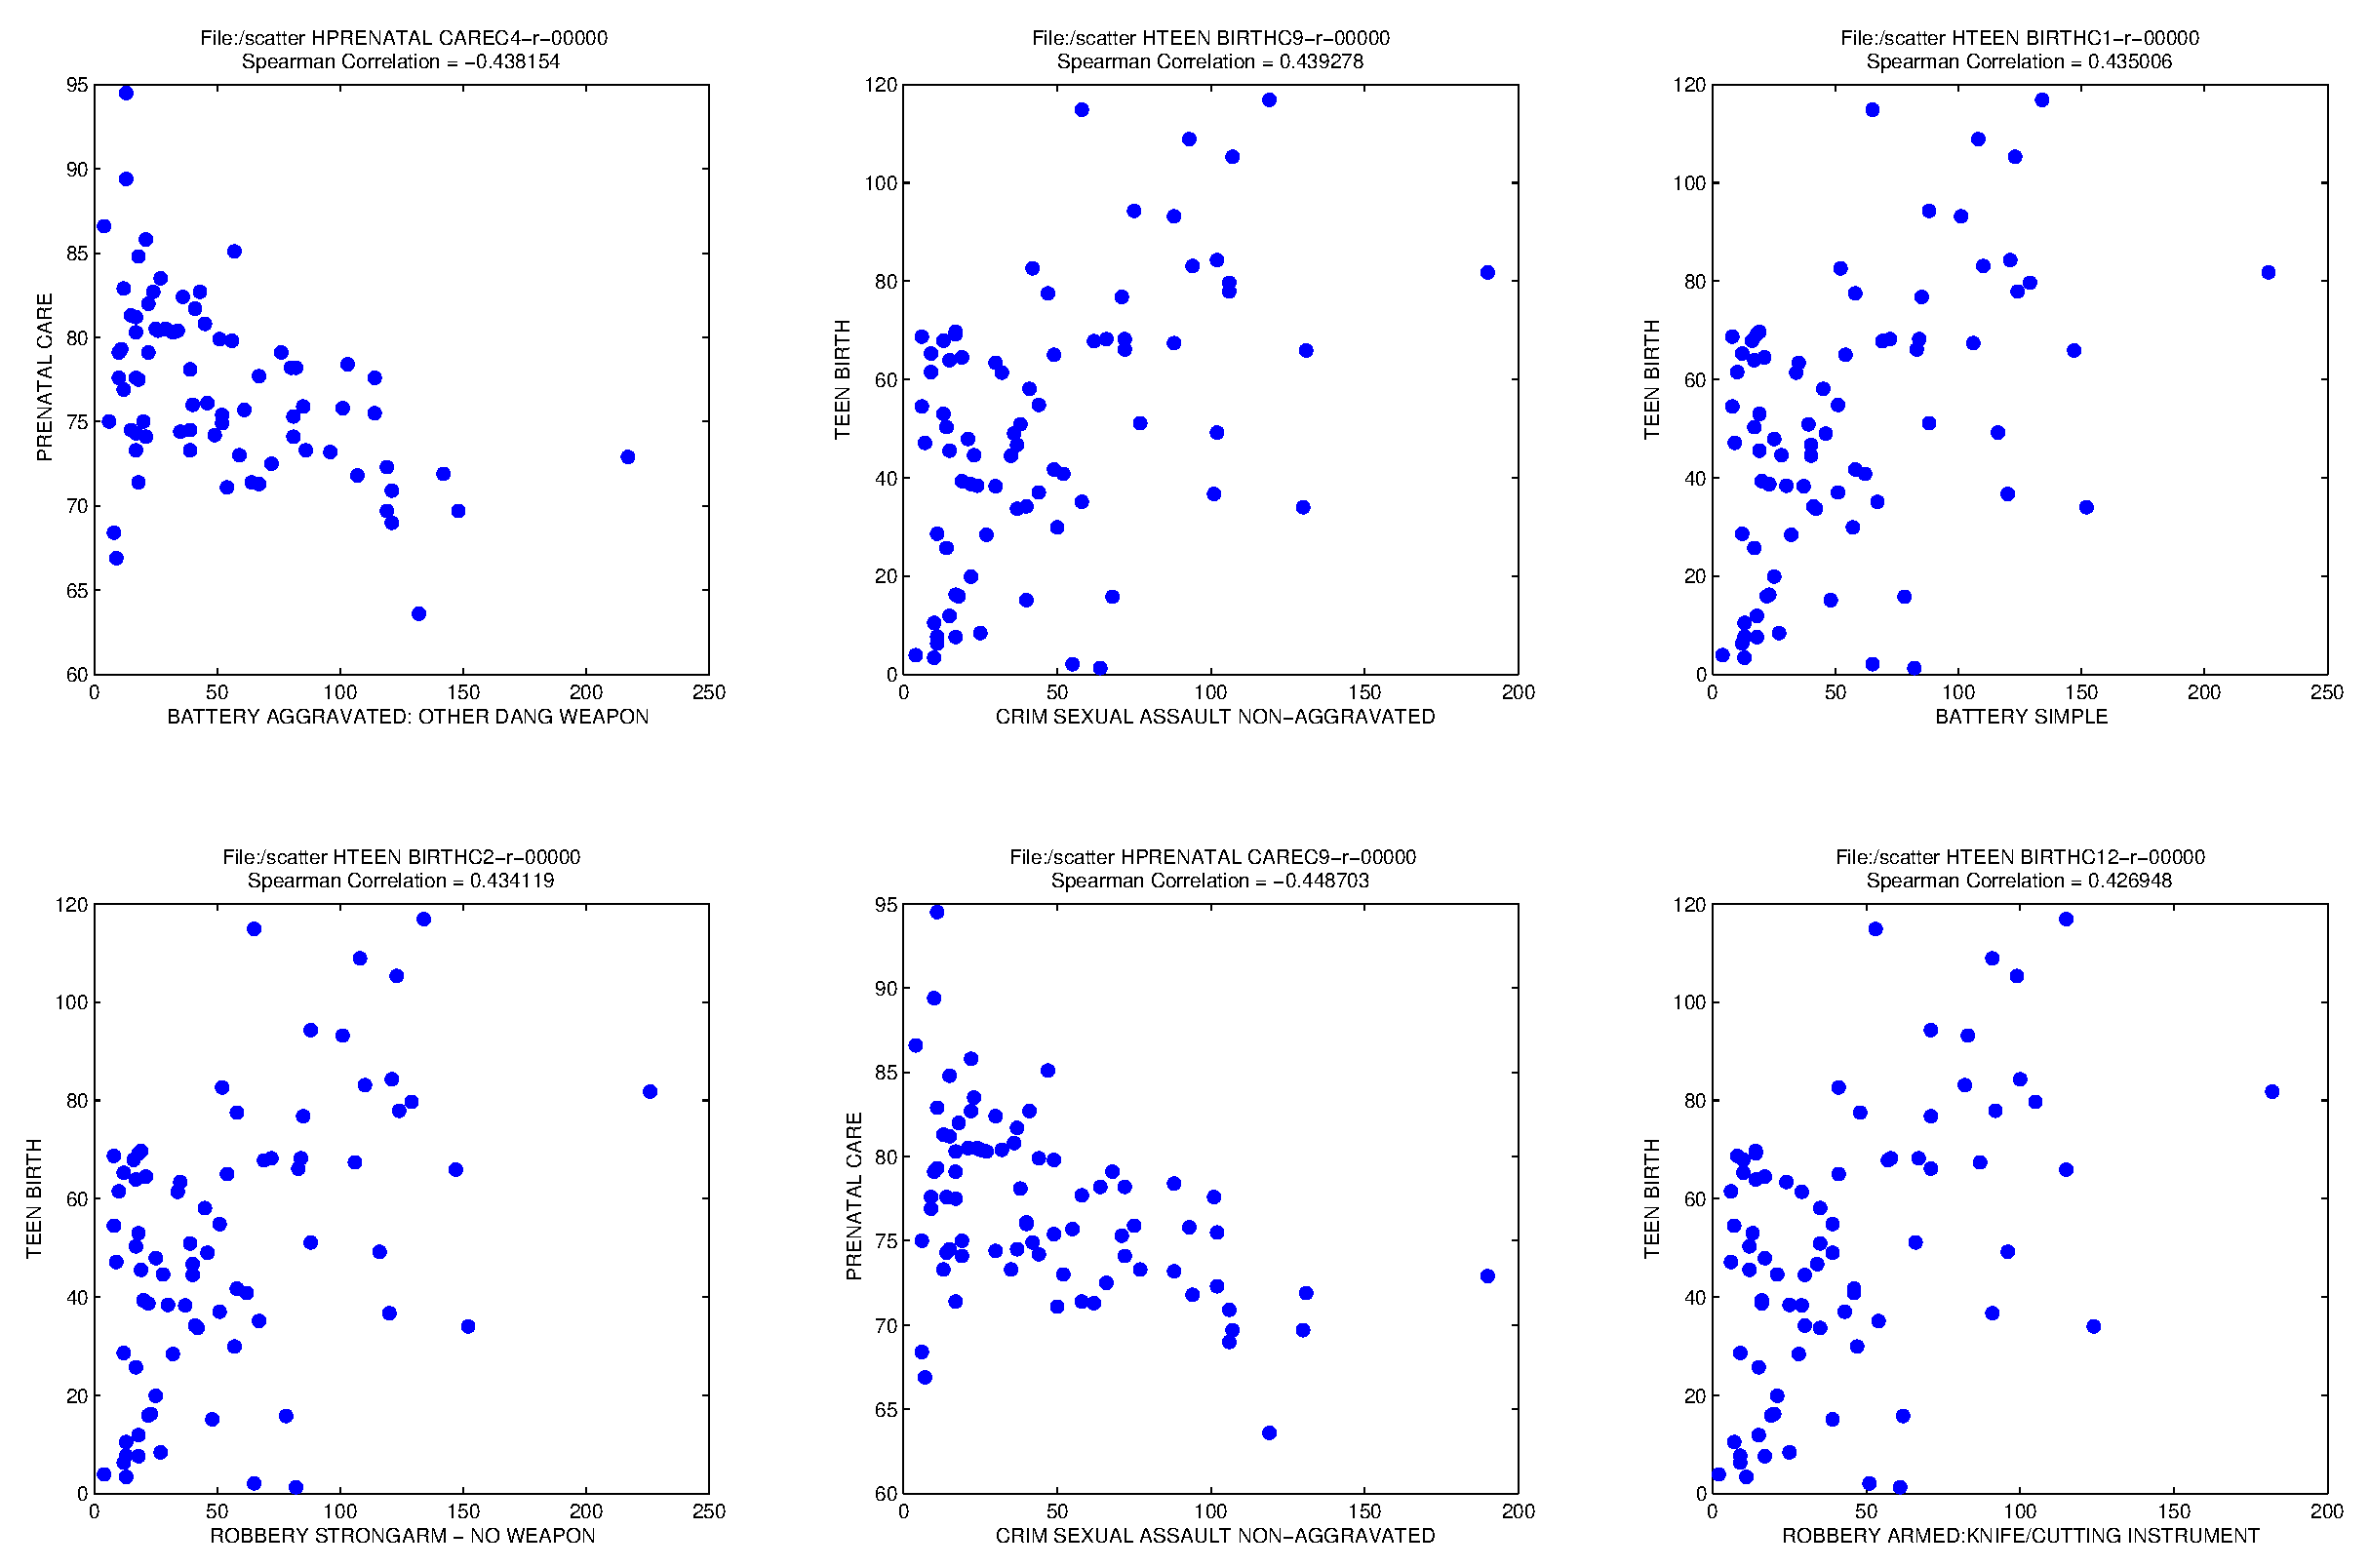
\includegraphics[width=0.3\linewidth]{media/ScatterPlot5.eps}
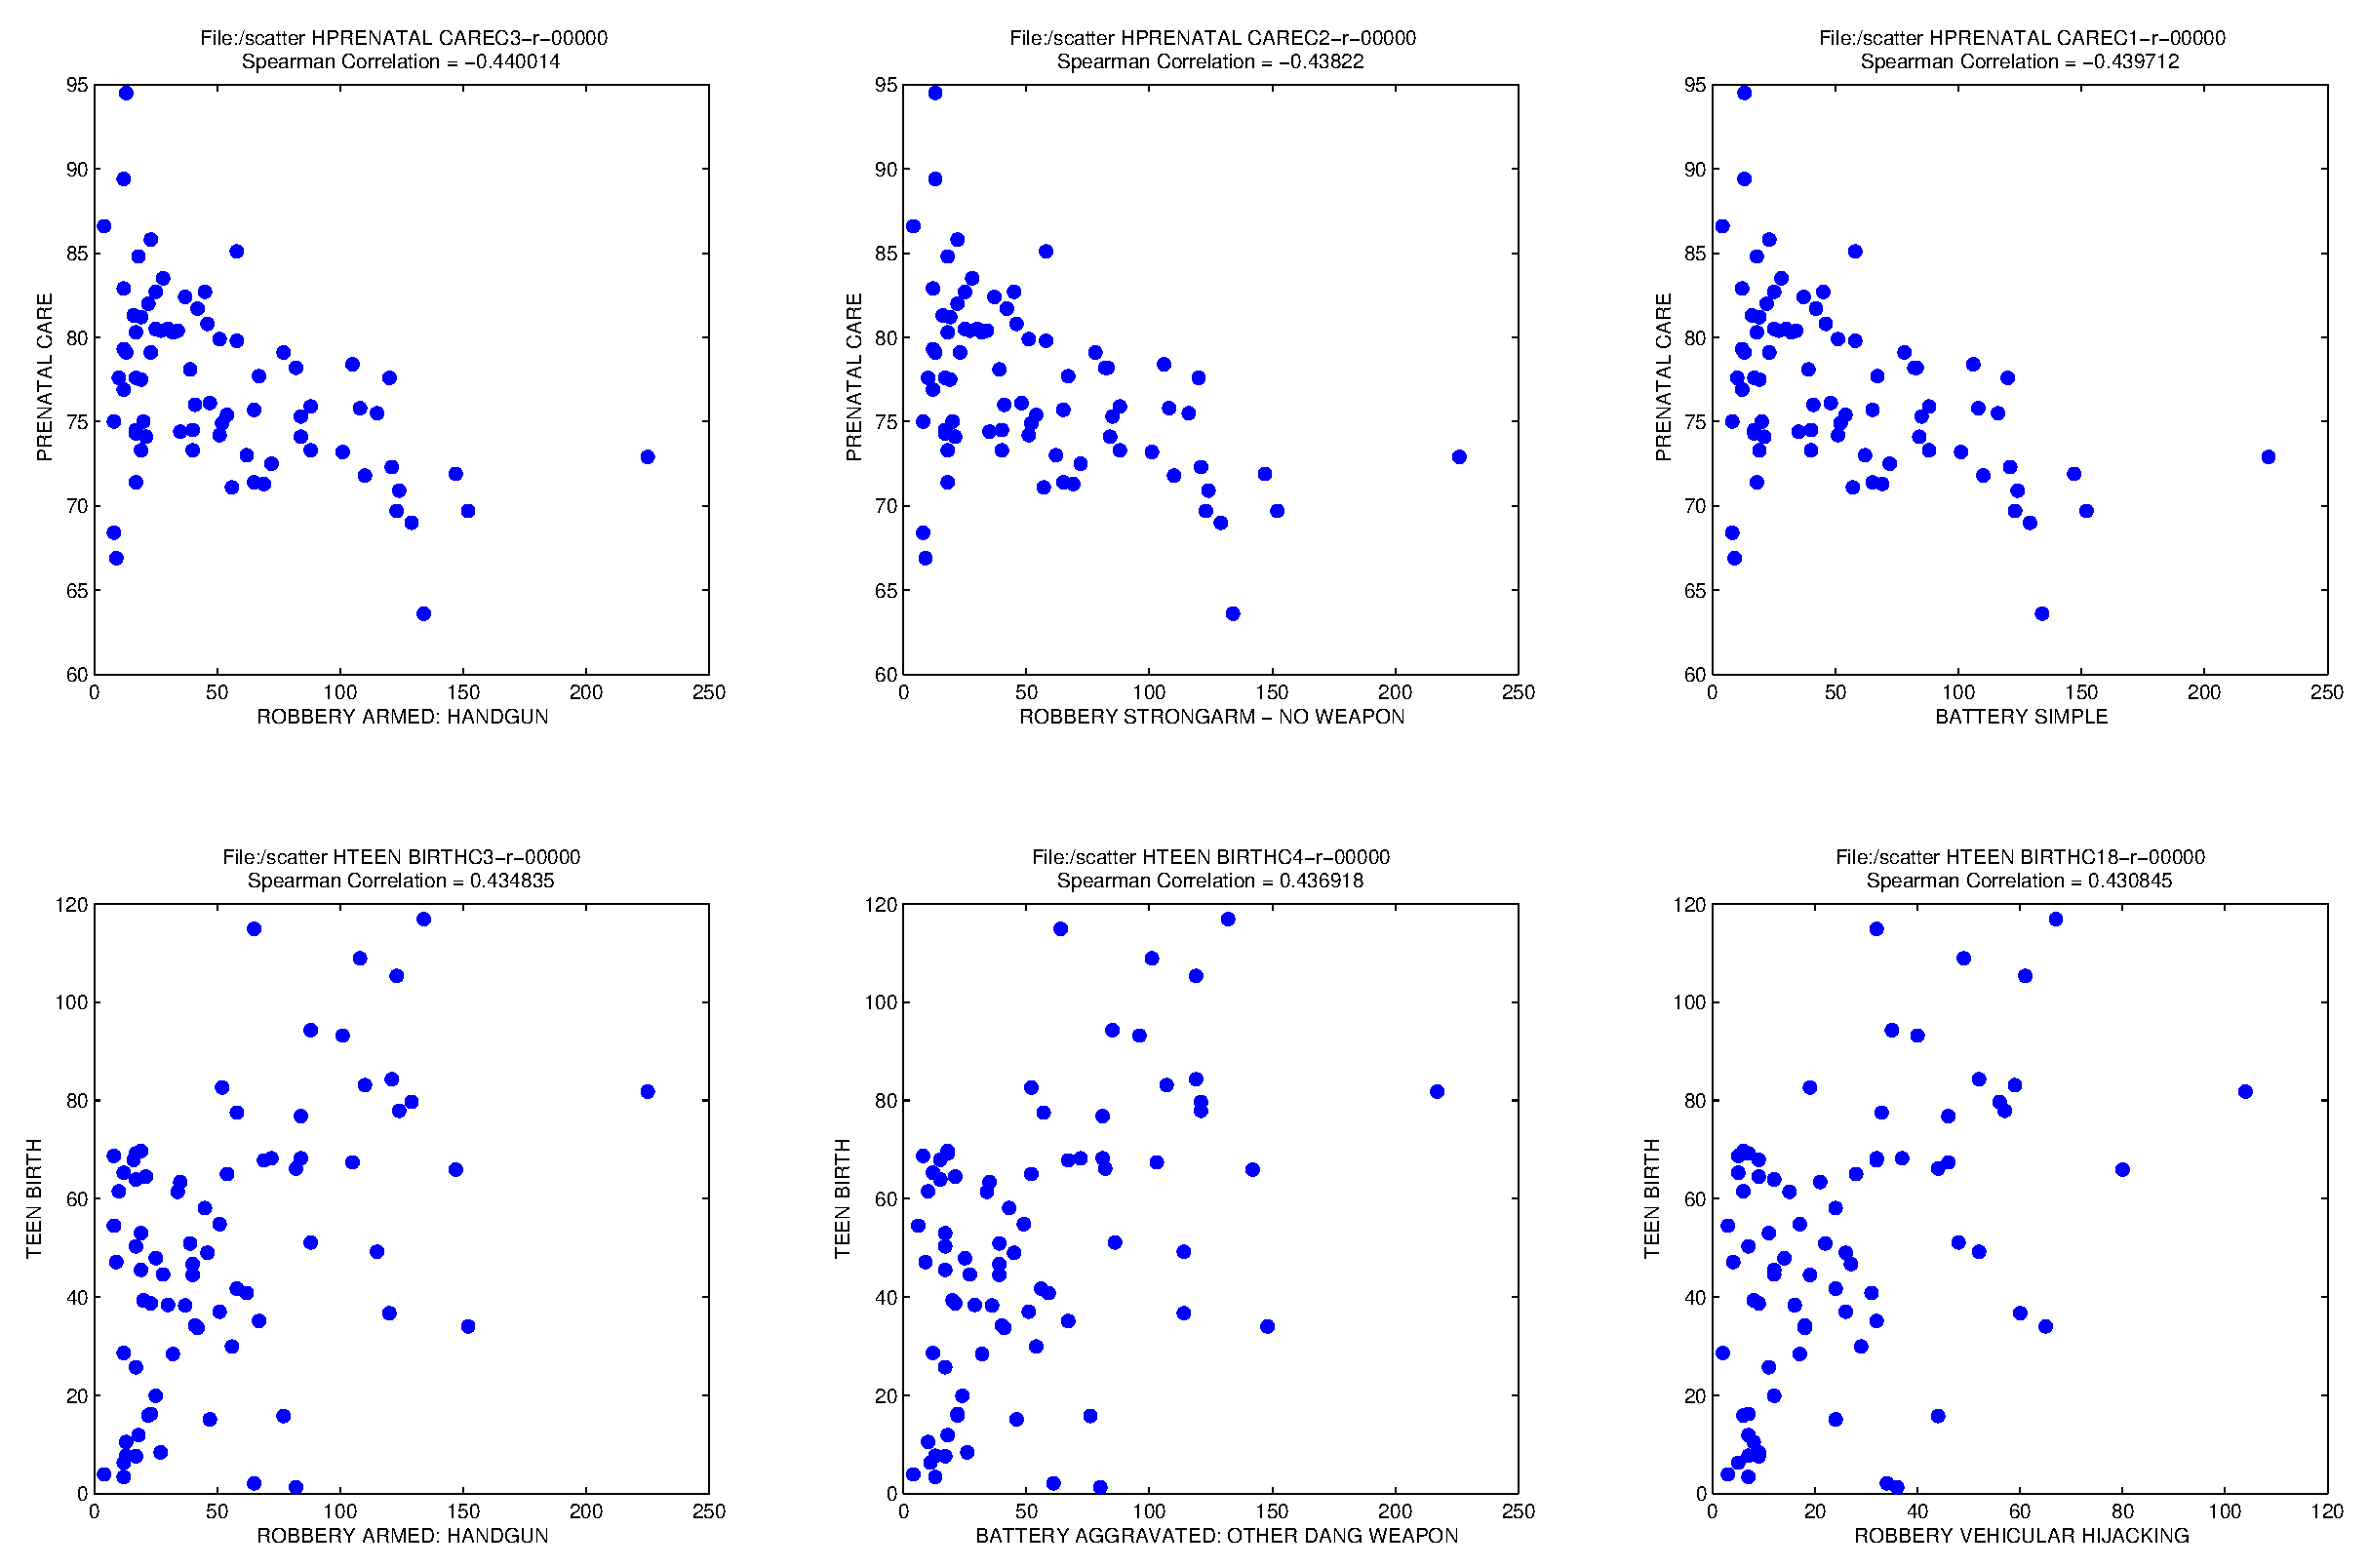
\includegraphics[width=0.3\linewidth]{media/ScatterPlot6.eps}
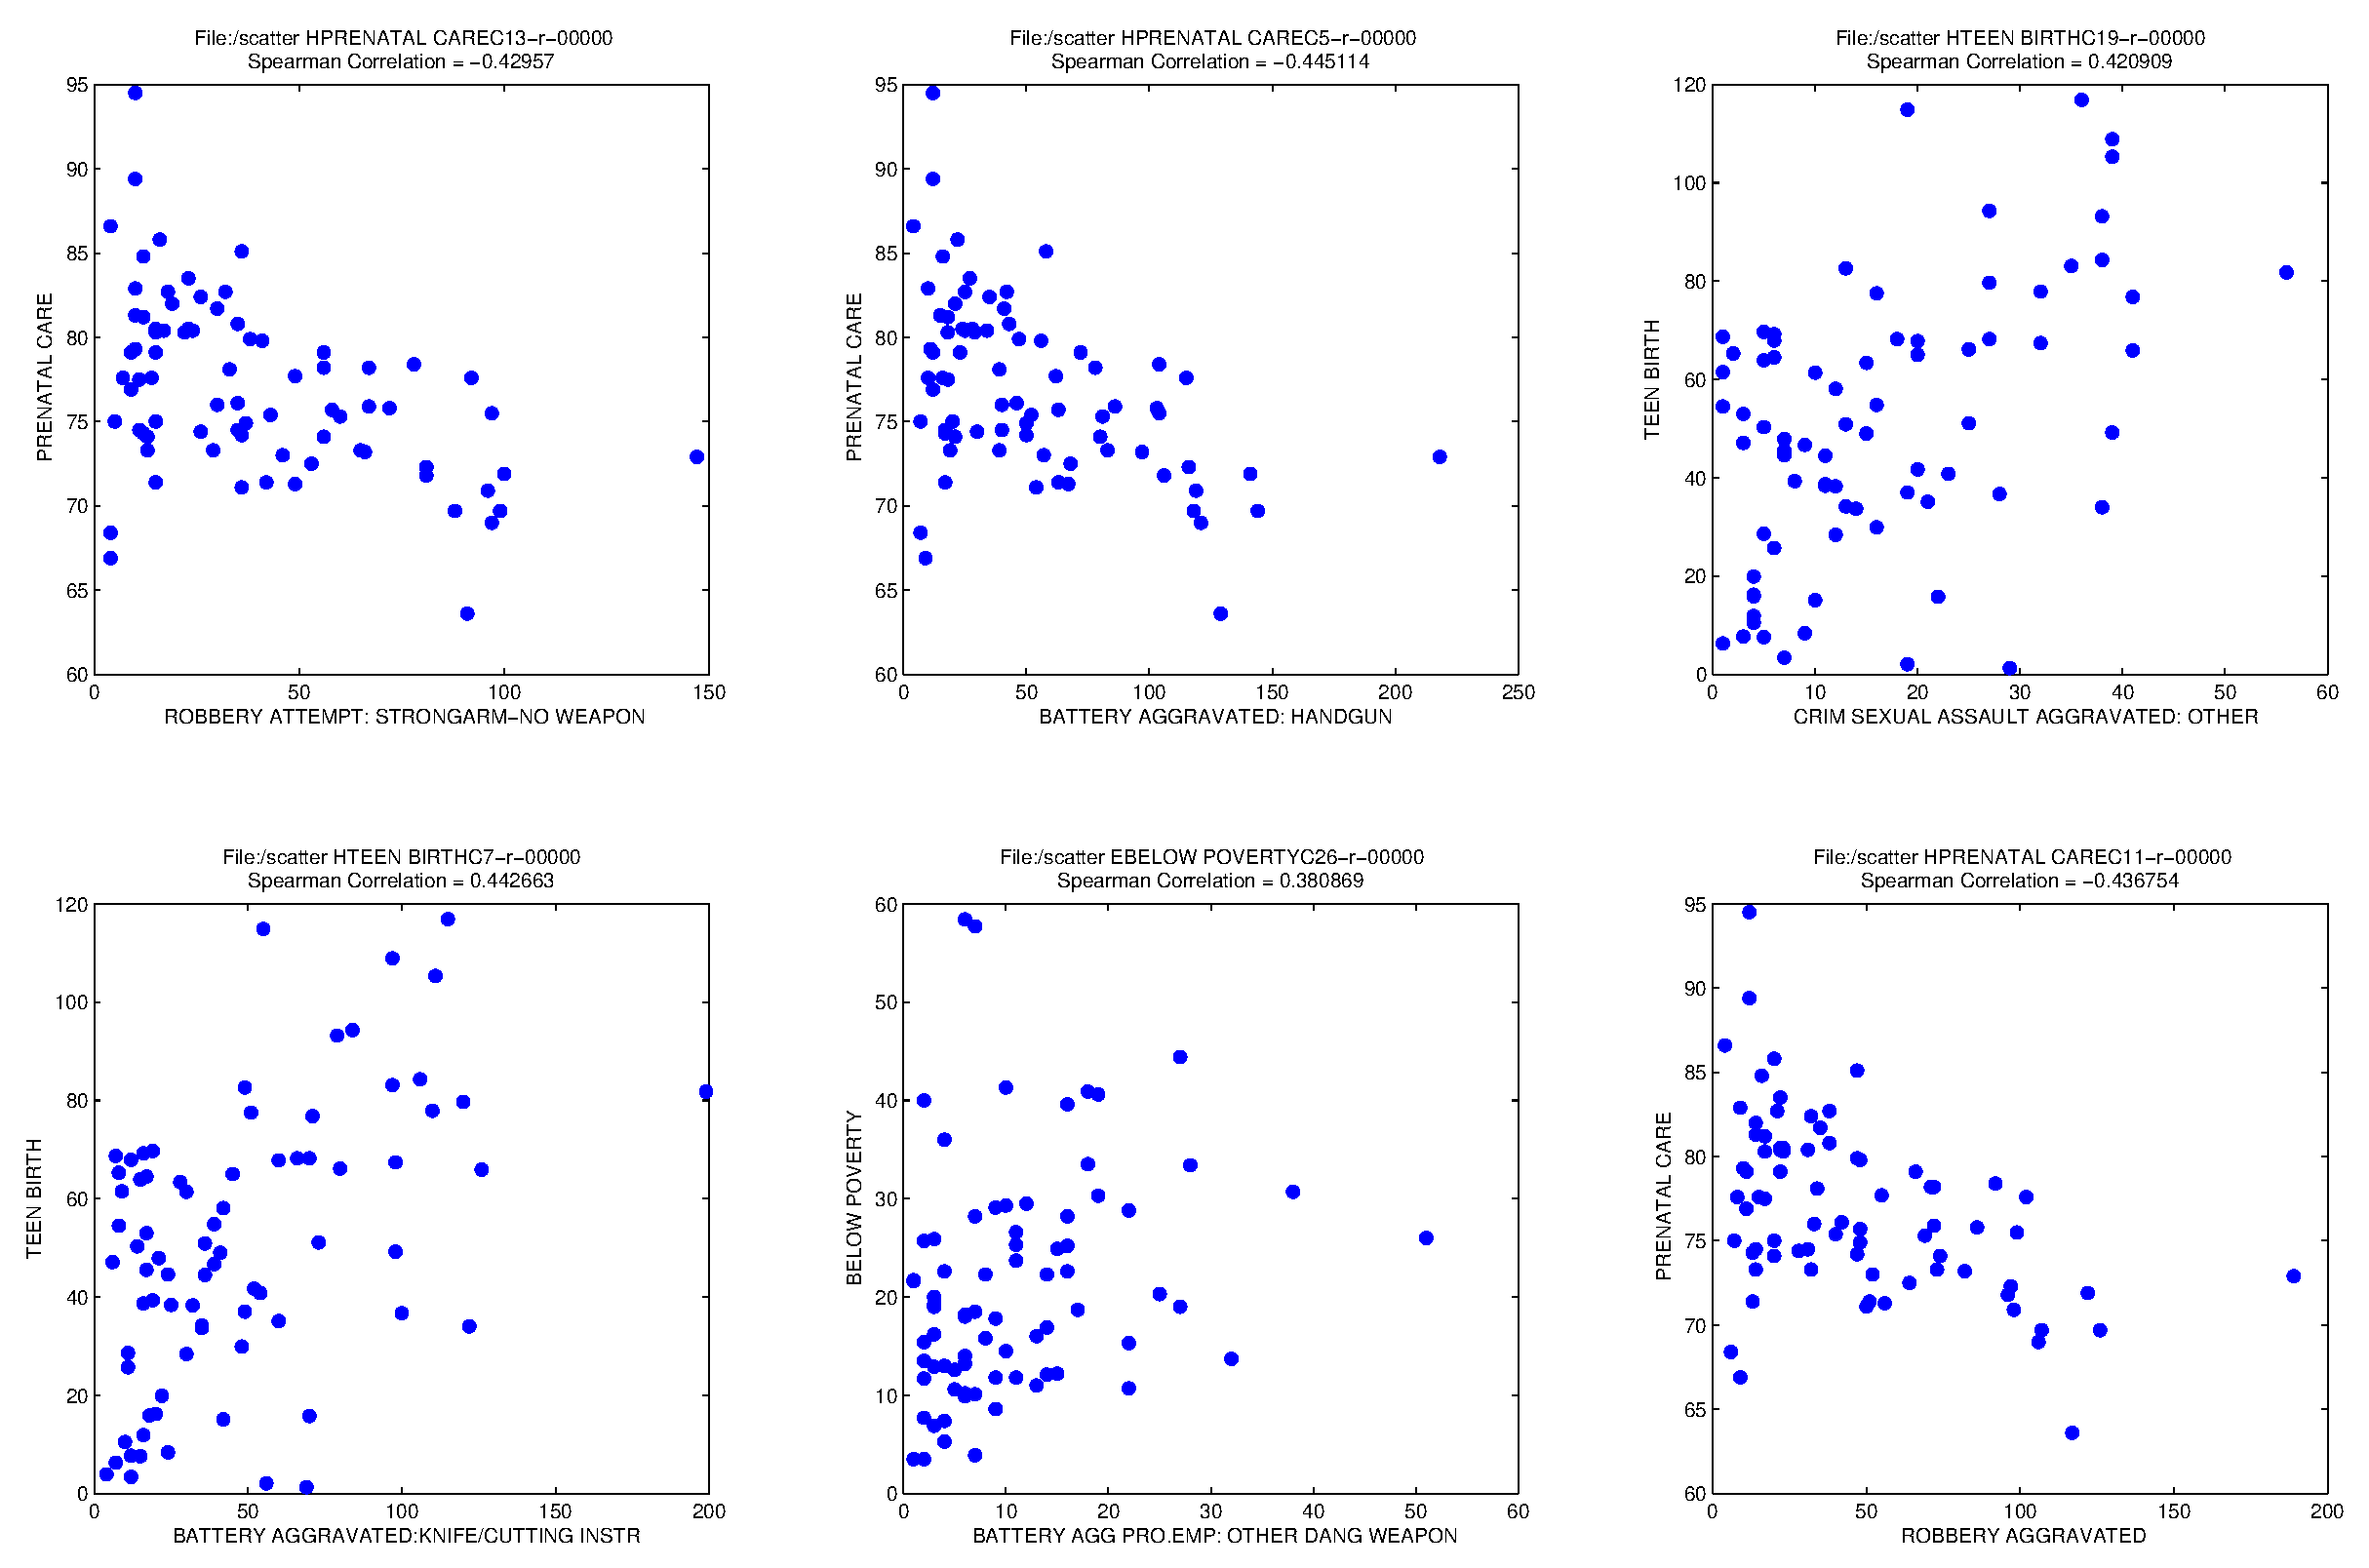
\includegraphics[width=0.3\linewidth]{media/ScatterPlot7.eps}
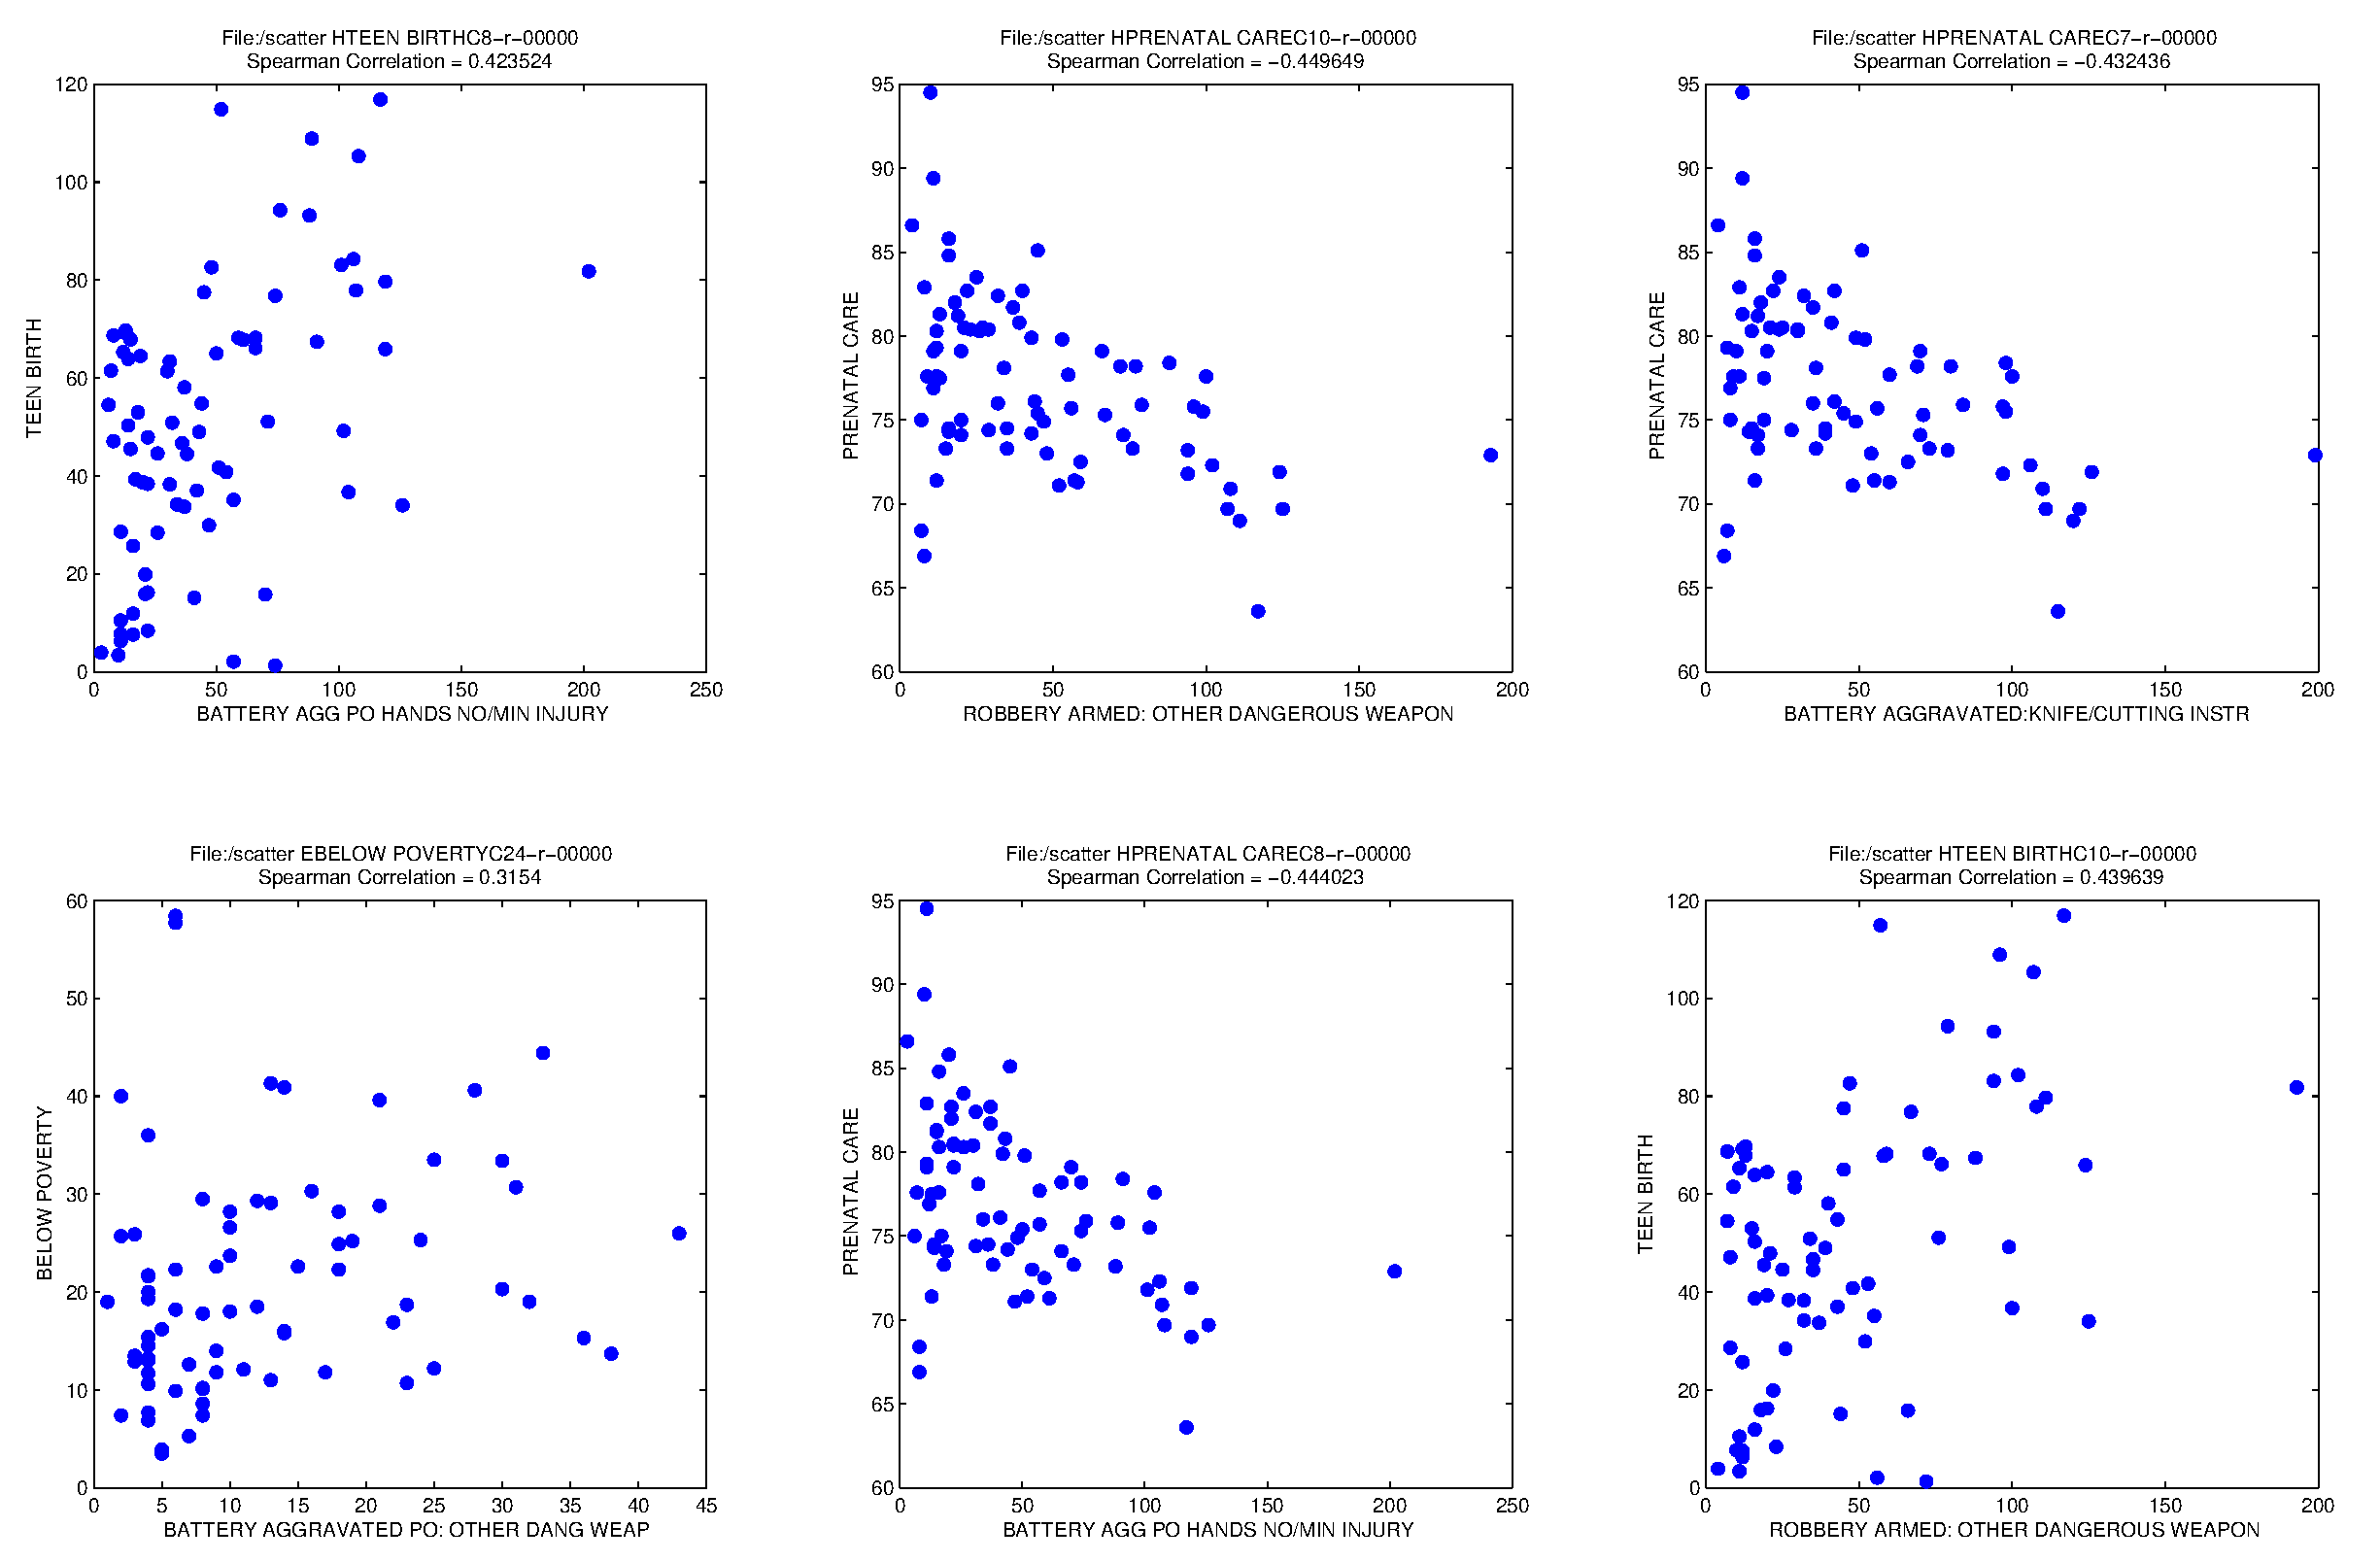
\includegraphics[width=0.3\linewidth]{media/ScatterPlot8.eps}\hspace{1cm}
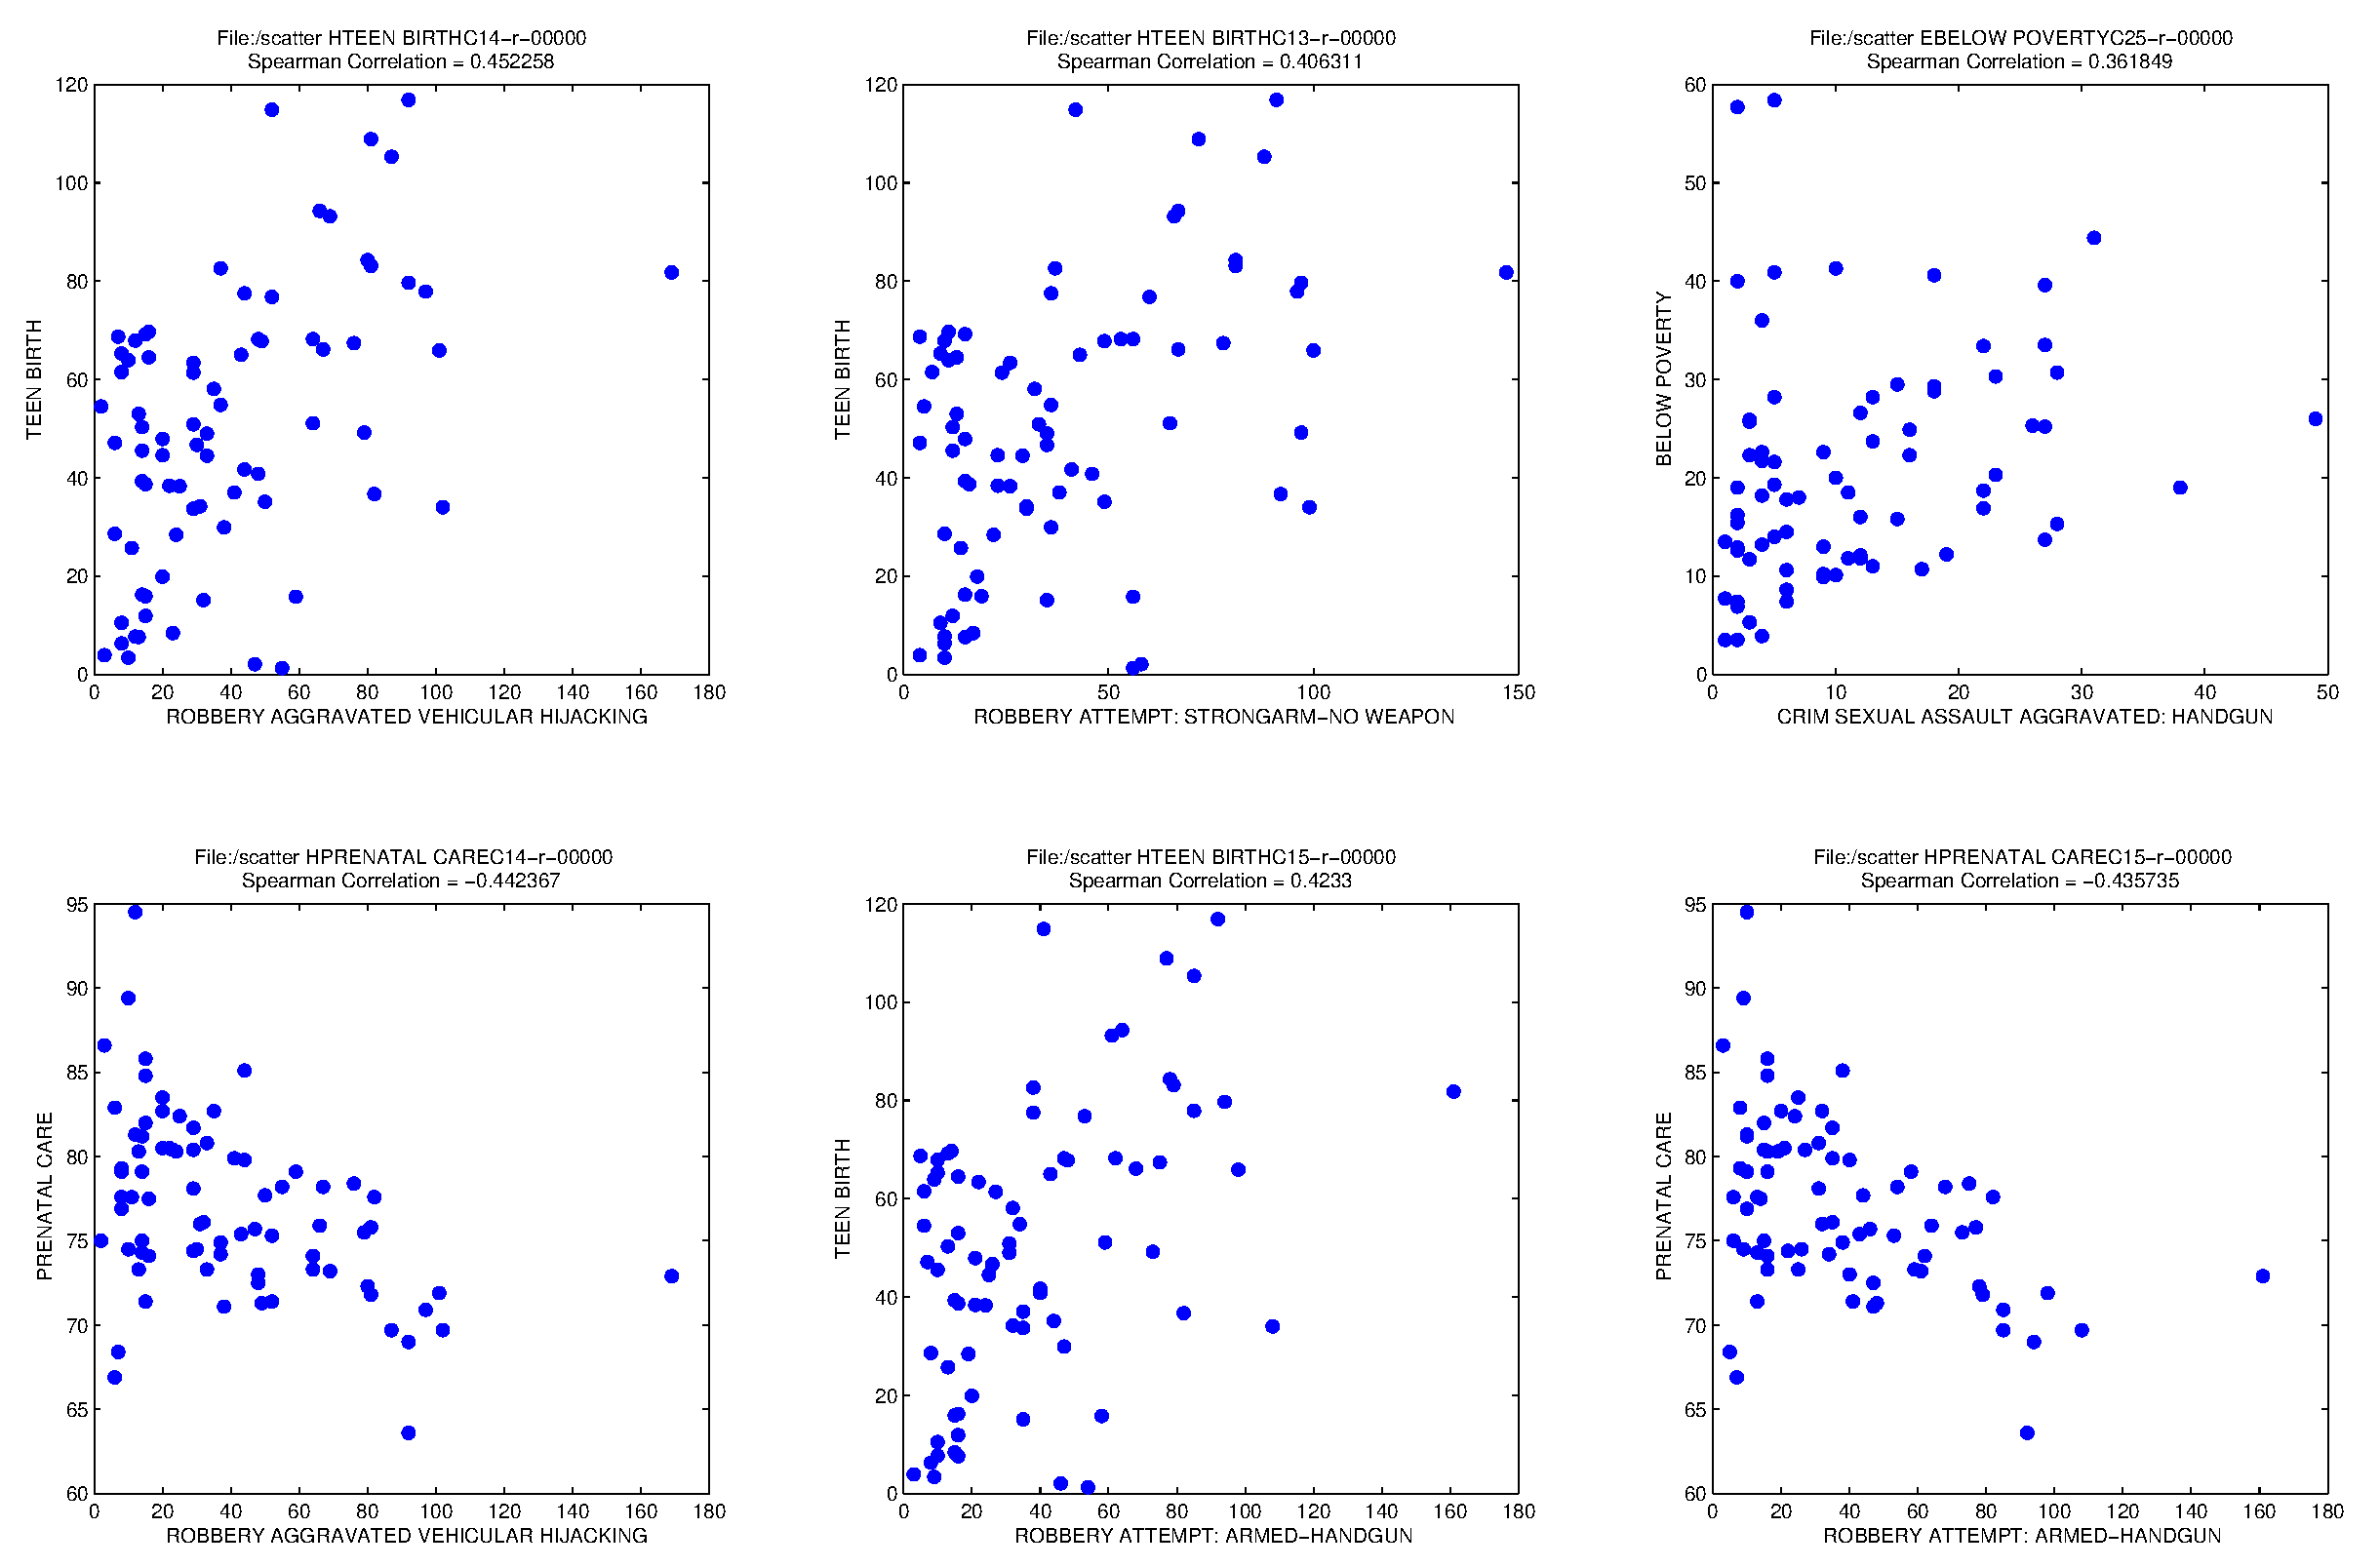
\includegraphics[width=0.3\linewidth]{media/ScatterPlot9.eps}
\caption{Scatter plots and Spearman Correlation}
\end{figure}

Out of the top 50 crimes, we chose to group them in three main groups: \textbf{Battery}, \textbf{Sexual Assault} and \textbf{Robberies}. Those crimes were the most frequent and we believed that they are different enough that a causal pattern was highly likely.

The distribution of the indicator values is described below.

\begin{figure}[ht]
	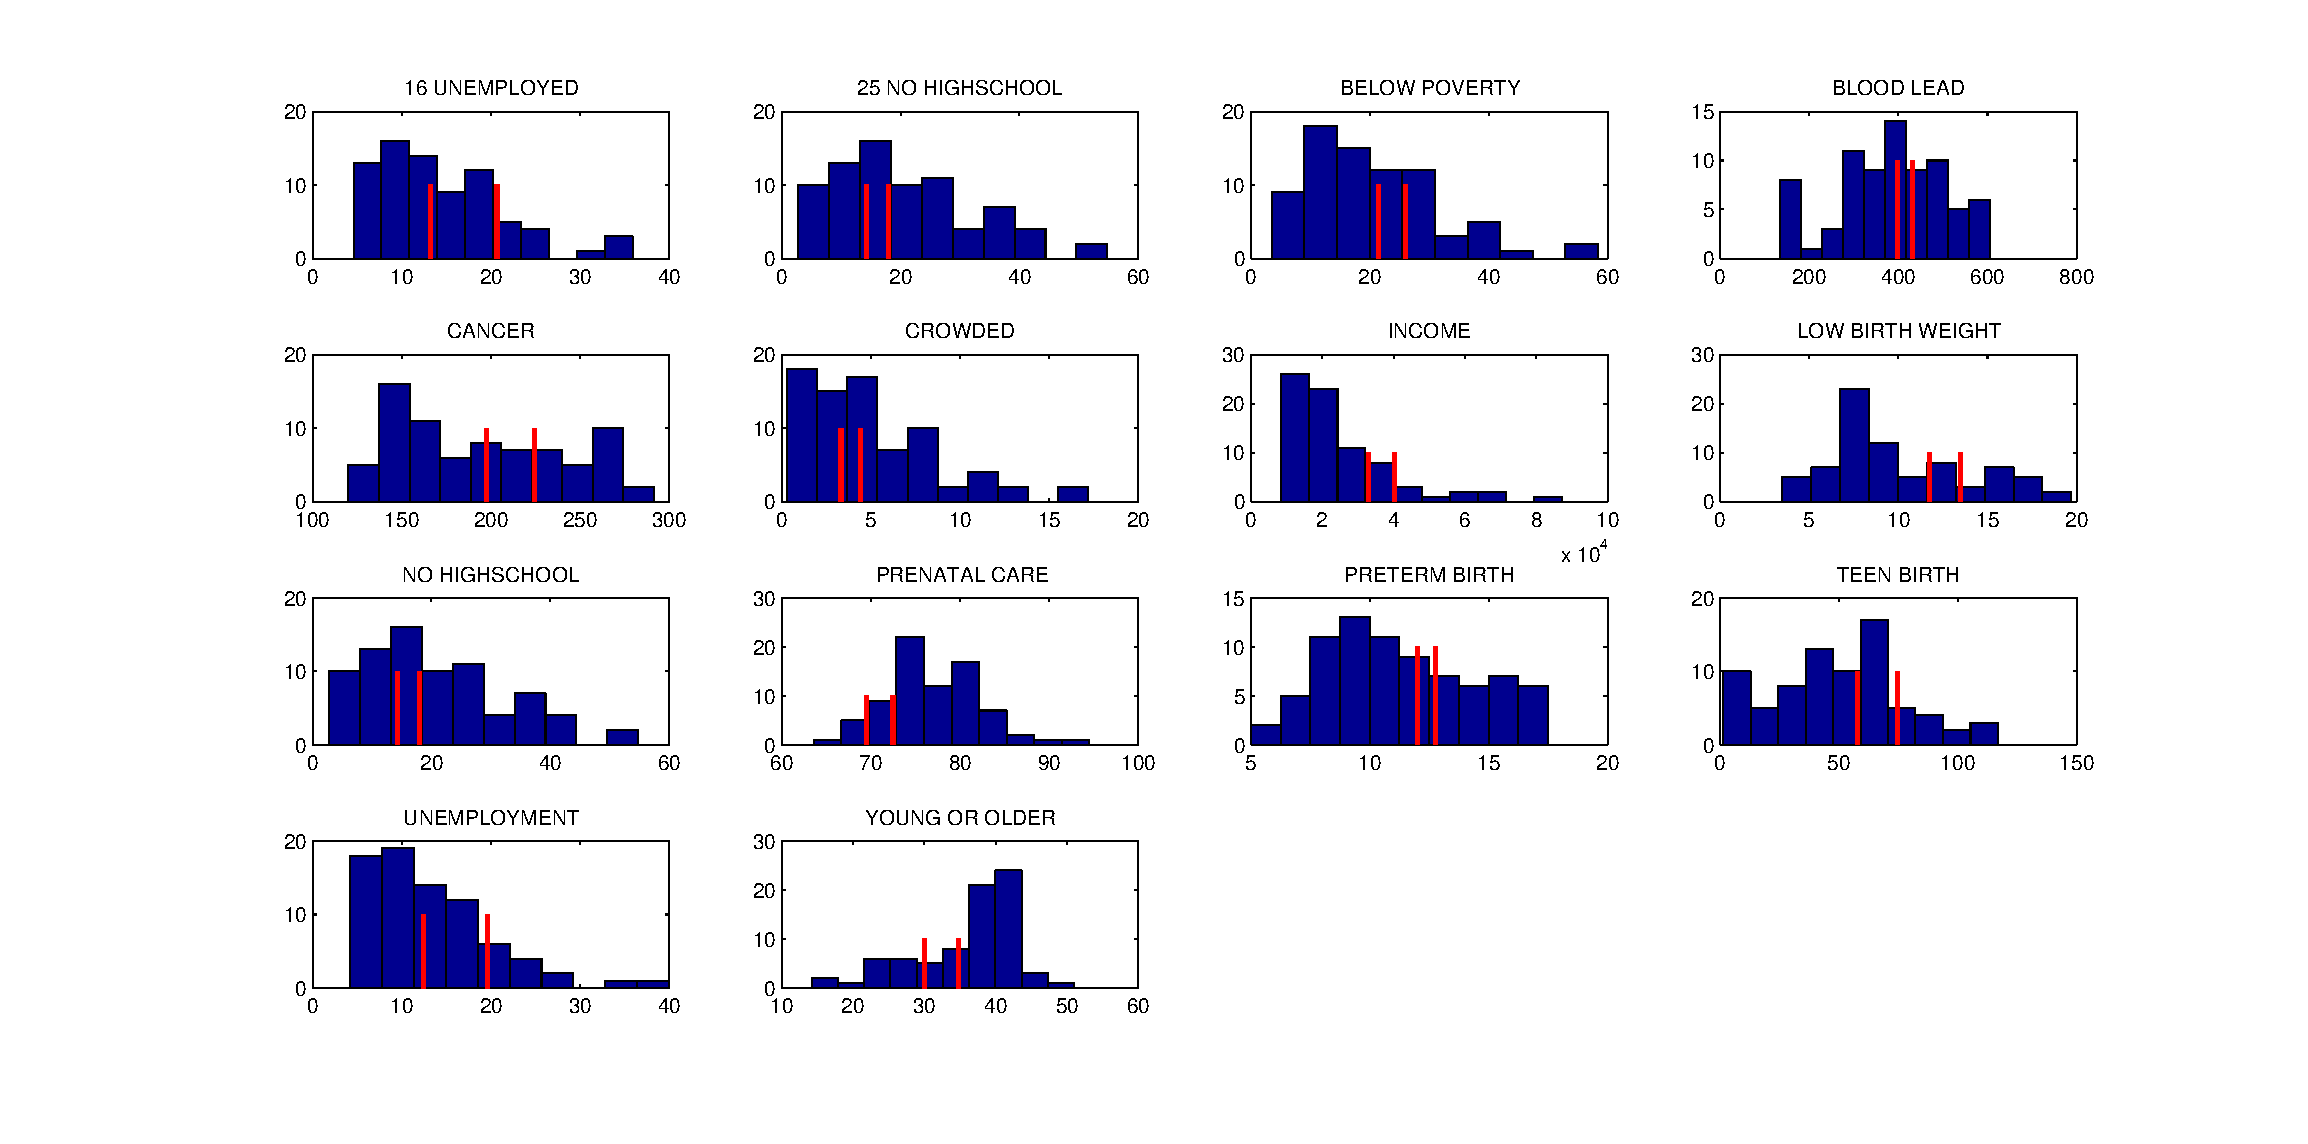
\includegraphics[width=\linewidth]{media/distribution.eps}
	\caption{Distribution of predictor variables. Lines in red represent the mean of the top 5 community areas with the highest type of crime for the three categories (BATTERY, SEXUAL ASSAULT, ROBBERY).}
\end{figure}

Based on these observations, we proceeded to generate artificial samples from the mean values of the indicators for each crime type. The algorithm is described below:

\begin{enumerate}
	\item Identify which group a given indicator belongs to (BATTERY, SEXUAL ASSAULT, ROBBERY).
	\item Extract the mean of the top 5 values for said indicator
	\item Create a sample with these values.
\end{enumerate}

These steps are performed on every one of the top 50 crimes, and then the data is used as training for a classification tree.

\begin{figure}[H]
	\includegraphics[width=\linewidth]{media/tree.eps}
	\caption{Classification tree based on three columns, INCOME, \% BELOW POVERTY and UNEMPLOYMENT}
\end{figure}

\section{Results}

We can see that the there are different variables that interact and that there is no single indicator that can predict the likelihood of a type of crime. While the interpretation of these results are highly subjective and only reflect a statistical correlation, much less an actual causation, we can conclude that certain indicators related to poverty are highly correlated with violent crime.\\

Specifically, we see that looking at the percentage of people below the poverty line, income level and unemployment of a specific community area, we can characterize the type of crimes that are most likely to occur.\\

An alternative tree using all the indicators provides the following result:

\begin{figure}[H]
	\centering
	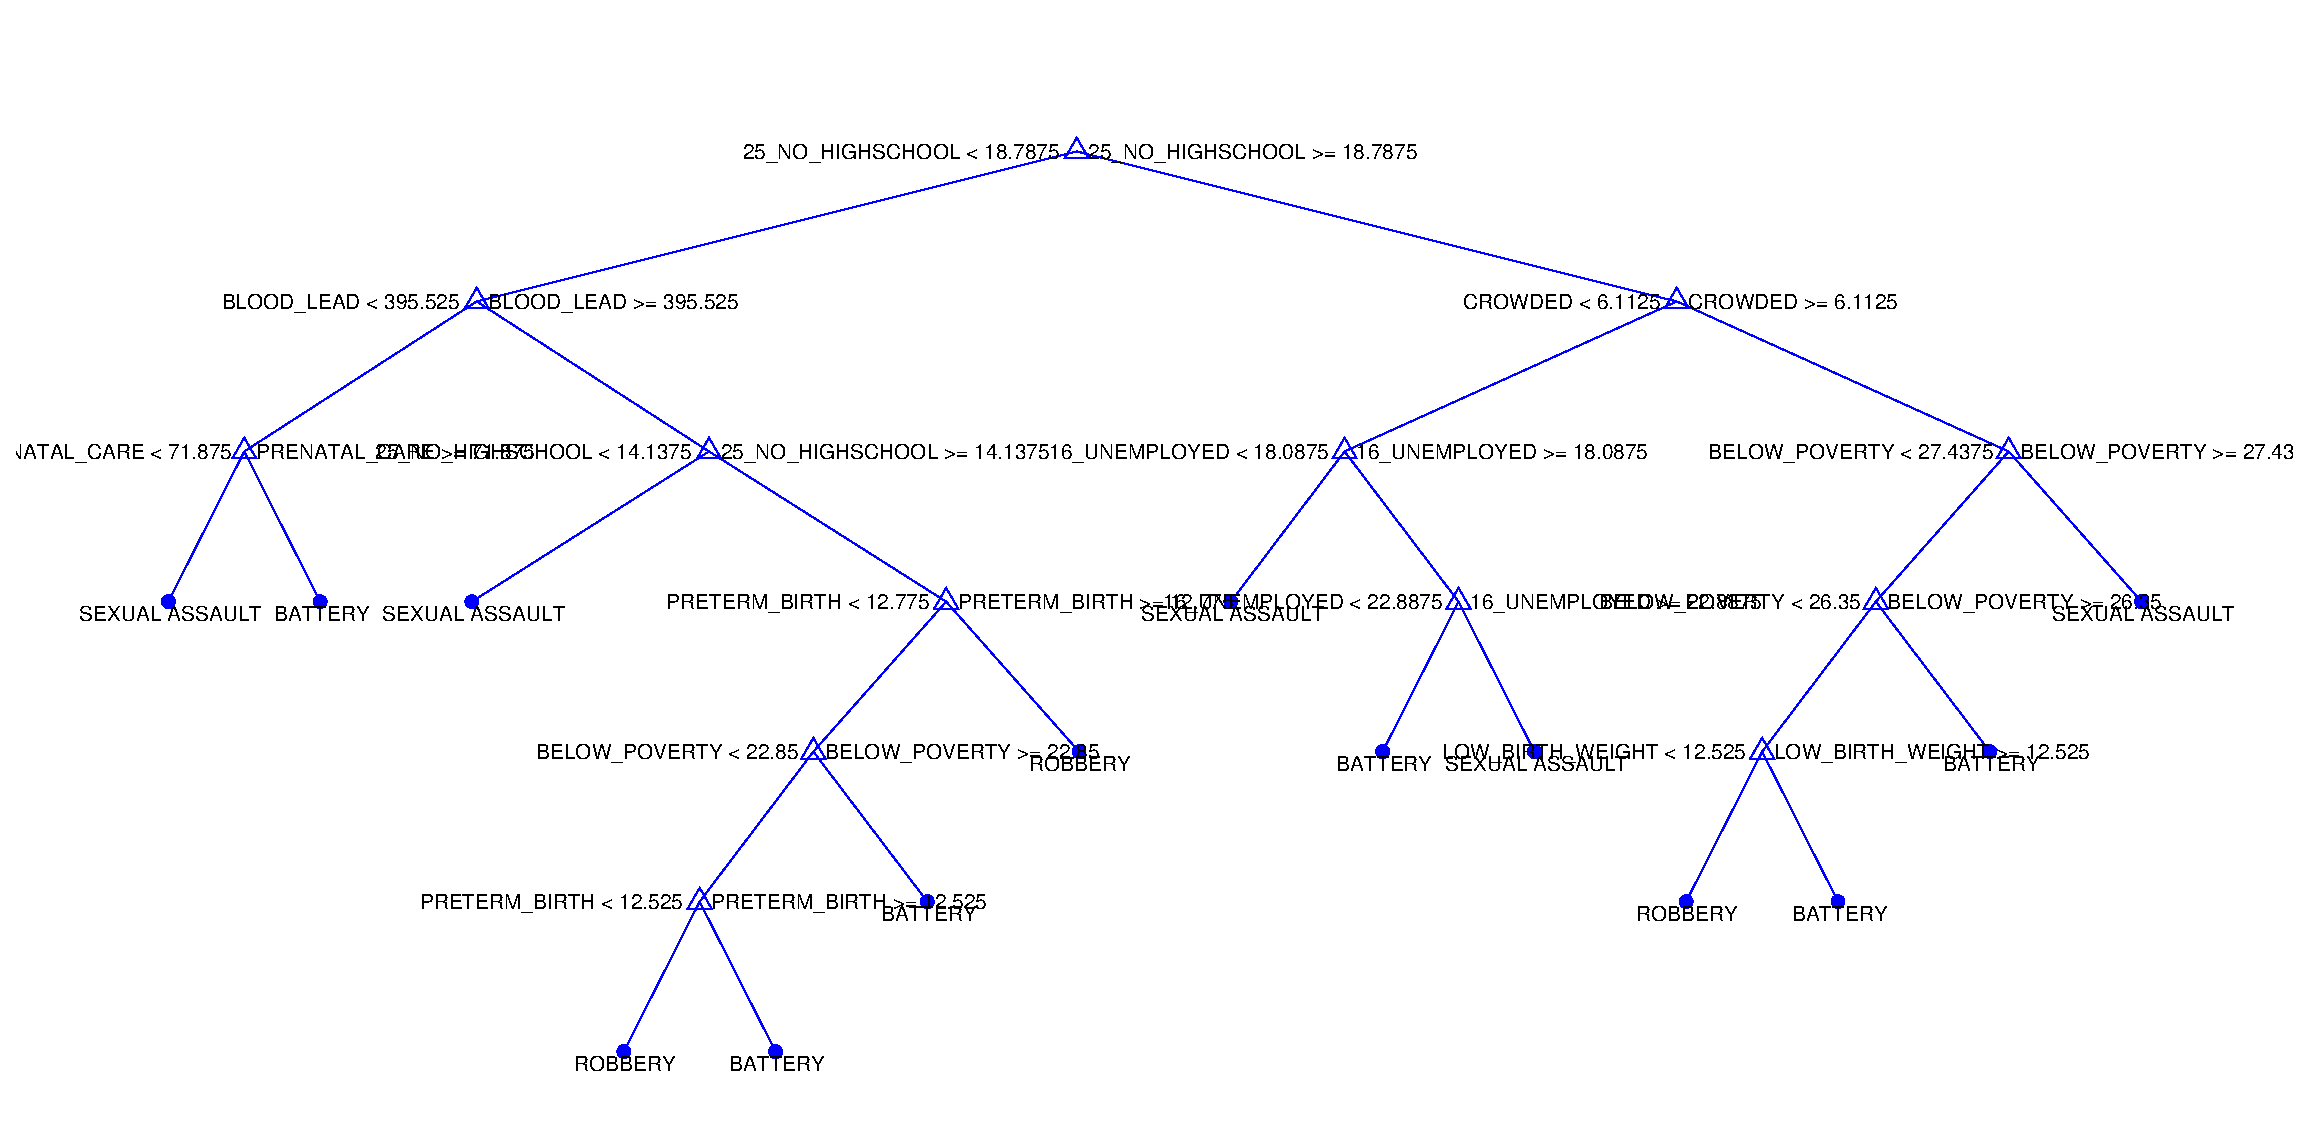
\includegraphics[width=0.6\linewidth]{media/full_tree.eps}
	\caption{Tree using all socio-economic indicators (Tree has been pruned)}
\end{figure}

\subsection{Future Work}

These project didn't perform a class-weighted classification, that is, homicides for example represent less than 2\% of all crime committed in Chicago, and therefore the classification technique used didn't capture the under-represented classes, missing them completely.
Another future improvement would include Montecarlo simulations to approximate the uncertainty in both the sample class and the indicators. These socio-economic and health indicators are sampled from a whole community area and local variability should be accounted for. Same for the sample classes: we are assuming that the crime classification for robbery is always accurate when different kinds of robberies related crimes could be analysed separately.


\section{Conclusion}

The process involved in putting this project together was very educational and we learned new techniques and familiarized ourselves even further with working on large datasets. We gained one of the more valuable gems of experience by reaching a dead end with our first attempt and rebuilding most things from scratch on a new dataset. There was also quite a bit of “peripheral data science” that needed to be done with various small programs that performed necessary operations, like the mapping of crimes to community area and other related activities which provided excellent learning opportunities.\\

In conclusion, we were able to use the MapReduce paradigm for data analytics like we had never done before. We truly enjoyed this class, as well as this project.

\newpage

\bibliographystyle{plain}
\bibliography{bibliography}

\end{document}
